
%% bare_conf.tex
%% V1.4a
%% 2014/09/17
%% by Michael Shell
%% See:
%% http://www.michaelshell.org/
%% for current contact information.
%%
%% This is a skeleton file demonstrating the use of IEEEtran.cls
%% (requires IEEEtran.cls version 1.8a or later) with an IEEE
%% conference paper.
%%
%% Support sites:
%% http://www.michaelshell.org/tex/ieeetran/
%% http://www.ctan.org/tex-archive/macros/latex/contrib/IEEEtran/
%% and
%% http://www.ieee.org/

% ================= IF YOU HAVE QUESTIONS =======================
% For questions regarding the IEEE styles, IEEE policies and
% procedures, conferences etc. please go to the IEEE web page at
% http://www.ieee.org/publications_standards/publications/authors
%
% Technical questions to bbob@lri.fr
% ===============================================================


%%*************************************************************************
%% Legal Notice:
%% This code is offered as-is without any warranty either expressed or
%% implied; without even the implied warranty of MERCHANTABILITY or
%% FITNESS FOR A PARTICULAR PURPOSE! 
%% User assumes all risk.
%% In no event shall IEEE or any contributor to this code be liable for
%% any damages or losses, including, but not limited to, incidental,
%% consequential, or any other damages, resulting from the use or misuse
%% of any information contained here.
%%
%% All comments are the opinions of their respective authors and are not
%% necessarily endorsed by the IEEE.
%%
%% This work is distributed under the LaTeX Project Public License (LPPL)
%% ( http://www.latex-project.org/ ) version 1.3, and may be freely used,
%% distributed and modified. A copy of the LPPL, version 1.3, is included
%% in the base LaTeX documentation of all distributions of LaTeX released
%% 2003/12/01 or later.
%% Retain all contribution notices and credits.
%% ** Modified files should be clearly indicated as such, including  **
%% ** renaming them and changing author support contact information. **
%%
%% File list of work: IEEEtran.cls, IEEEtran_HOWTO.pdf, bare_adv.tex,
%%                    bare_conf.tex, bare_jrnl.tex, bare_conf_compsoc.tex,
%%                    bare_jrnl_compsoc.tex, bare_jrnl_transmag.tex
%%*************************************************************************


% *** Authors should verify (and, if needed, correct) their LaTeX system  ***
% *** with the testflow diagnostic prior to trusting their LaTeX platform ***
% *** with production work. IEEE's font choices and paper sizes can       ***
% *** trigger bugs that do not appear when using other class files.       ***                          ***
% The testflow support page is at:
% http://www.michaelshell.org/tex/testflow/



\documentclass[conference]{IEEEtran}
% Some Computer Society conferences also require the compsoc mode option,
% but others use the standard conference format.
%
% If IEEEtran.cls has not been installed into the LaTeX system files,
% manually specify the path to it like:
% \documentclass[conference]{../sty/IEEEtran}

\usepackage{graphicx}
\usepackage{tabularx}
\usepackage[dvipsnames]{xcolor}
\usepackage{float}
\usepackage{rotating}
\usepackage{xstring} % for string operations
\usepackage{wasysym} % Table legend with symbols input from post-processing
\usepackage{savesym} % needed to rename \iint and \iint definitions in order to load them from MnSymbol library rather than from amsmath
\savesymbol{iint}
\savesymbol{iiint}
\usepackage{MnSymbol} % Table legend with symbols input from post-processing




% Some very useful LaTeX packages include:
% (uncomment the ones you want to load)


% *** MISC UTILITY PACKAGES ***
%
%\usepackage{ifpdf}
% Heiko Oberdiek's ifpdf.sty is very useful if you need conditional
% compilation based on whether the output is pdf or dvi.
% usage:
% \ifpdf
%   % pdf code
% \else
%   % dvi code
% \fi
% The latest version of ifpdf.sty can be obtained from:
% http://www.ctan.org/tex-archive/macros/latex/contrib/oberdiek/
% Also, note that IEEEtran.cls V1.7 and later provides a builtin
% \ifCLASSINFOpdf conditional that works the same way.
% When switching from latex to pdflatex and vice-versa, the compiler may
% have to be run twice to clear warning/error messages.






% *** CITATION PACKAGES ***
%
%\usepackage{cite}
% cite.sty was written by Donald Arseneau
% V1.6 and later of IEEEtran pre-defines the format of the cite.sty package
% \cite{} output to follow that of IEEE. Loading the cite package will
% result in citation numbers being automatically sorted and properly
% "compressed/ranged". e.g., [1], [9], [2], [7], [5], [6] without using
% cite.sty will become [1], [2], [5]--[7], [9] using cite.sty. cite.sty's
% \cite will automatically add leading space, if needed. Use cite.sty's
% noadjust option (cite.sty V3.8 and later) if you want to turn this off
% such as if a citation ever needs to be enclosed in parenthesis.
% cite.sty is already installed on most LaTeX systems. Be sure and use
% version 5.0 (2009-03-20) and later if using hyperref.sty.
% The latest version can be obtained at:
% http://www.ctan.org/tex-archive/macros/latex/contrib/cite/
% The documentation is contained in the cite.sty file itself.






% *** GRAPHICS RELATED PACKAGES ***
%
\ifCLASSINFOpdf
  % \usepackage[pdftex]{graphicx}
  % declare the path(s) where your graphic files are
  % \graphicspath{{../pdf/}{../jpeg/}}
  % and their extensions so you won't have to specify these with
  % every instance of \includegraphics
  % \DeclareGraphicsExtensions{.pdf,.jpeg,.png}
\else
  % or other class option (dvipsone, dvipdf, if not using dvips). graphicx
  % will default to the driver specified in the system graphics.cfg if no
  % driver is specified.
  % \usepackage[dvips]{graphicx}
  % declare the path(s) where your graphic files are
  % \graphicspath{{../eps/}}
  % and their extensions so you won't have to specify these with
  % every instance of \includegraphics
  % \DeclareGraphicsExtensions{.eps}
\fi
% graphicx was written by David Carlisle and Sebastian Rahtz. It is
% required if you want graphics, photos, etc. graphicx.sty is already
% installed on most LaTeX systems. The latest version and documentation
% can be obtained at: 
% http://www.ctan.org/tex-archive/macros/latex/required/graphics/
% Another good source of documentation is "Using Imported Graphics in
% LaTeX2e" by Keith Reckdahl which can be found at:
% http://www.ctan.org/tex-archive/info/epslatex/
%
% latex, and pdflatex in dvi mode, support graphics in encapsulated
% postscript (.eps) format. pdflatex in pdf mode supports graphics
% in .pdf, .jpeg, .png and .mps (metapost) formats. Users should ensure
% that all non-photo figures use a vector format (.eps, .pdf, .mps) and
% not a bitmapped formats (.jpeg, .png). IEEE frowns on bitmapped formats
% which can result in "jaggedy"/blurry rendering of lines and letters as
% well as large increases in file sizes.
%
% You can find documentation about the pdfTeX application at:
% http://www.tug.org/applications/pdftex





% *** MATH PACKAGES ***
%
%\usepackage[cmex10]{amsmath}
% A popular package from the American Mathematical Society that provides
% many useful and powerful commands for dealing with mathematics. If using
% it, be sure to load this package with the cmex10 option to ensure that
% only type 1 fonts will utilized at all point sizes. Without this option,
% it is possible that some math symbols, particularly those within
% footnotes, will be rendered in bitmap form which will result in a
% document that can not be IEEE Xplore compliant!
%
% Also, note that the amsmath package sets \interdisplaylinepenalty to 10000
% thus preventing page breaks from occurring within multiline equations. Use:
%\interdisplaylinepenalty=2500
% after loading amsmath to restore such page breaks as IEEEtran.cls normally
% does. amsmath.sty is already installed on most LaTeX systems. The latest
% version and documentation can be obtained at:
% http://www.ctan.org/tex-archive/macros/latex/required/amslatex/math/





% *** SPECIALIZED LIST PACKAGES ***
%
%\usepackage{algorithmic}
% algorithmic.sty was written by Peter Williams and Rogerio Brito.
% This package provides an algorithmic environment fo describing algorithms.
% You can use the algorithmic environment in-text or within a figure
% environment to provide for a floating algorithm. Do NOT use the algorithm
% floating environment provided by algorithm.sty (by the same authors) or
% algorithm2e.sty (by Christophe Fiorio) as IEEE does not use dedicated
% algorithm float types and packages that provide these will not provide
% correct IEEE style captions. The latest version and documentation of
% algorithmic.sty can be obtained at:
% http://www.ctan.org/tex-archive/macros/latex/contrib/algorithms/
% There is also a support site at:
% http://algorithms.berlios.de/index.html
% Also of interest may be the (relatively newer and more customizable)
% algorithmicx.sty package by Szasz Janos:
% http://www.ctan.org/tex-archive/macros/latex/contrib/algorithmicx/




% *** ALIGNMENT PACKAGES ***
%
%\usepackage{array}
% Frank Mittelbach's and David Carlisle's array.sty patches and improves
% the standard LaTeX2e array and tabular environments to provide better
% appearance and additional user controls. As the default LaTeX2e table
% generation code is lacking to the point of almost being broken with
% respect to the quality of the end results, all users are strongly
% advised to use an enhanced (at the very least that provided by array.sty)
% set of table tools. array.sty is already installed on most systems. The
% latest version and documentation can be obtained at:
% http://www.ctan.org/tex-archive/macros/latex/required/tools/


% IEEEtran contains the IEEEeqnarray family of commands that can be used to
% generate multiline equations as well as matrices, tables, etc., of high
% quality.




% *** SUBFIGURE PACKAGES ***
%\ifCLASSOPTIONcompsoc
%  \usepackage[caption=false,font=normalsize,labelfont=sf,textfont=sf]{subfig}
%\else
%  \usepackage[caption=false,font=footnotesize]{subfig}
%\fi
% subfig.sty, written by Steven Douglas Cochran, is the modern replacement
% for subfigure.sty, the latter of which is no longer maintained and is
% incompatible with some LaTeX packages including fixltx2e. However,
% subfig.sty requires and automatically loads Axel Sommerfeldt's caption.sty
% which will override IEEEtran.cls' handling of captions and this will result
% in non-IEEE style figure/table captions. To prevent this problem, be sure
% and invoke subfig.sty's "caption=false" package option (available since
% subfig.sty version 1.3, 2005/06/28) as this is will preserve IEEEtran.cls
% handling of captions.
% Note that the Computer Society format requires a larger sans serif font
% than the serif footnote size font used in traditional IEEE formatting
% and thus the need to invoke different subfig.sty package options depending
% on whether compsoc mode has been enabled.
%
% The latest version and documentation of subfig.sty can be obtained at:
% http://www.ctan.org/tex-archive/macros/latex/contrib/subfig/




% *** FLOAT PACKAGES ***
%
%\usepackage{fixltx2e}
% fixltx2e, the successor to the earlier fix2col.sty, was written by
% Frank Mittelbach and David Carlisle. This package corrects a few problems
% in the LaTeX2e kernel, the most notable of which is that in current
% LaTeX2e releases, the ordering of single and double column floats is not
% guaranteed to be preserved. Thus, an unpatched LaTeX2e can allow a
% single column figure to be placed prior to an earlier double column
% figure. The latest version and documentation can be found at:
% http://www.ctan.org/tex-archive/macros/latex/base/


%\usepackage{stfloats}
% stfloats.sty was written by Sigitas Tolusis. This package gives LaTeX2e
% the ability to do double column floats at the bottom of the page as well
% as the top. (e.g., "\begin{figure*}[!b]" is not normally possible in
% LaTeX2e). It also provides a command:
%\fnbelowfloat
% to enable the placement of footnotes below bottom floats (the standard
% LaTeX2e kernel puts them above bottom floats). This is an invasive package
% which rewrites many portions of the LaTeX2e float routines. It may not work
% with other packages that modify the LaTeX2e float routines. The latest
% version and documentation can be obtained at:
% http://www.ctan.org/tex-archive/macros/latex/contrib/sttools/
% Do not use the stfloats baselinefloat ability as IEEE does not allow
% \baselineskip to stretch. Authors submitting work to the IEEE should note
% that IEEE rarely uses double column equations and that authors should try
% to avoid such use. Do not be tempted to use the cuted.sty or midfloat.sty
% packages (also by Sigitas Tolusis) as IEEE does not format its papers in
% such ways.
% Do not attempt to use stfloats with fixltx2e as they are incompatible.
% Instead, use Morten Hogholm'a dblfloatfix which combines the features
% of both fixltx2e and stfloats:
%
% \usepackage{dblfloatfix}
% The latest version can be found at:
% http://www.ctan.org/tex-archive/macros/latex/contrib/dblfloatfix/




% *** PDF, URL AND HYPERLINK PACKAGES ***
%
%\usepackage{url}
% url.sty was written by Donald Arseneau. It provides better support for
% handling and breaking URLs. url.sty is already installed on most LaTeX
% systems. The latest version and documentation can be obtained at:
% http://www.ctan.org/tex-archive/macros/latex/contrib/url/
% Basically, \url{my_url_here}.




% *** Do not adjust lengths that control margins, column widths, etc. ***
% *** Do not use packages that alter fonts (such as pslatex).         ***
% There should be no need to do such things with IEEEtran.cls V1.6 and later.
% (Unless specifically asked to do so by the journal or conference you plan
% to submit to, of course. )


%%%%%%%%%%%%%%%%%%%%%%%%%%%%%%%%%%%%%%%%%%%%%%%%%%%%%%
% Definitions

% Algorithm names on the right of the ECDF figures can be modified by
% uncommenting the following lines and inputting some text in the last
% brackets, make sure the algorithms are in the same order as for the post-processing:
% \newcommand{\algaperfprof}{Algorithm a short name}
% \newcommand{\algbperfprof}{Algorithm b short name}
% \newcommand{\algcperfprof}{Algorithm c short name}
% \newcommand{\algdperfprof}{Algorithm c short name}
% ...
% Algorithm names as they appear in the tables, uncomment if necessary
% \newcommand{\algatables}{\algaperfprof}  % first argument in the post-processing
% \newcommand{\algbtables}{\algbperfprof}  % first argument in the post-processing
% \newcommand{\algctables}{\algcperfprof}  % first argument in the post-processing
% \newcommand{\algdtables}{\algdperfprof}  % second argument in the post-processing
% ...
% location of pictures files
\newcommand{\bbobdatapath}{ppdata/}
\input{\bbobdatapath bbob_pproc_commands.tex}
\graphicspath{{\bbobdatapath\algfolder}}
%
%%%%%%%%%%%%%%%%%%%%%%%%%%%%%%%%%%%%%%%%%%%%%%%%%%%%%%%
%% pre-defined commands
\newcommand{\DIM}{\ensuremath{\mathrm{DIM}}}
\newcommand{\ERT}{\ensuremath{\mathrm{ERT}}}
\newcommand{\FEvals}{\ensuremath{\mathrm{FEvals}}}
\newcommand{\nruns}{\ensuremath{\mathrm{Nruns}}}
\newcommand{\Dfb}{\ensuremath{\Delta f_{\mathrm{best}}}}
\newcommand{\Df}{\ensuremath{\Delta f}}
\newcommand{\nbFEs}{\ensuremath{\mathrm{\#FEs}}}
\newcommand{\fopt}{\ensuremath{f_\mathrm{opt}}}
\newcommand{\ftarget}{\ensuremath{f_\mathrm{t}}}
\newcommand{\CrE}{\ensuremath{\mathrm{CrE}}}
\newcommand{\change}[1]{{\color{red} #1}}

    \renewcommand{\topfraction}{1}	% max fraction of floats at top
    \renewcommand{\bottomfraction}{1} % max fraction of floats at bottom
    %   Parameters for TEXT pages (not float pages):
    \setcounter{topnumber}{3}
    \setcounter{bottomnumber}{3}
    \setcounter{totalnumber}{3}     % 2 may work better
    \setcounter{dbltopnumber}{4}    % for 2-column pages
    \renewcommand{\dbltopfraction}{1}	% fit big float above 2-col. text
    \renewcommand{\textfraction}{0.0}	% allow minimal text w. figs
    %   Parameters for FLOAT pages (not text pages):
    \renewcommand{\floatpagefraction}{0.80}	% require fuller float pages
    % N.B.: floatpagefraction MUST be less than topfraction !!
    \renewcommand{\dblfloatpagefraction}{0.7}	% require fuller float pages

%%%%%%%%%%%%%%%%%%%%%%%%%%%%%%%%%%%%%%%%%%%%%%%%%%%%%%


% correct bad hyphenation here
\hyphenation{op-tical net-works semi-conduc-tor}


\begin{document}
%
% paper title
% Titles are generally capitalized except for words such as a, an, and, as,
% at, but, by, for, in, nor, of, on, or, the, to and up, which are usually
% not capitalized unless they are the first or last word of the title.
% Linebreaks \\ can be used within to get better formatting as desired.
% Do not put math or special symbols in the title.
\title{Black-Box Optimization Benchmarking Template for Noiseless Function Testbed\\ {\large Draft version}}

% author names and affiliations
% use a multiple column layout for up to three different
% affiliations
\author{\IEEEauthorblockN{Firstname Lastname}
\IEEEauthorblockA{Affiliation\\
Address\\
Email: youremail@yourinstitution.org}\thanks{Submission deadline: December 19, 2014.}
%\and
%\IEEEauthorblockN{Homer Simpson}
%\IEEEauthorblockA{Twentieth Century Fox\\
%Springfield, USA\\
%Email: homer@thesimpsons.com}
%\and
%\IEEEauthorblockN{James Kirk\\ and Montgomery Scott}
%\IEEEauthorblockA{Starfleet Academy\\
%San Francisco, California 96678-2391\\
%Telephone: (800) 555--1212\\
%Fax: (888) 555--1212}
}

% conference papers do not typically use \thanks and this command
% is locked out in conference mode. If really needed, such as for
% the acknowledgment of grants, issue a \IEEEoverridecommandlockouts
% after \documentclass
\IEEEoverridecommandlockouts

% for over three affiliations, or if they all won't fit within the width
% of the page, use this alternative format:
% 
%\author{\IEEEauthorblockN{Michael Shell\IEEEauthorrefmark{1},
%Homer Simpson\IEEEauthorrefmark{2},
%James Kirk\IEEEauthorrefmark{3}, 
%Montgomery Scott\IEEEauthorrefmark{3} and
%Eldon Tyrell\IEEEauthorrefmark{4}}
%\IEEEauthorblockA{\IEEEauthorrefmark{1}School of Electrical and Computer Engineering\\
%Georgia Institute of Technology,
%Atlanta, Georgia 30332--0250\\ Email: see http://www.michaelshell.org/contact.html}
%\IEEEauthorblockA{\IEEEauthorrefmark{2}Twentieth Century Fox, Springfield, USA\\
%Email: homer@thesimpsons.com}
%\IEEEauthorblockA{\IEEEauthorrefmark{3}Starfleet Academy, San Francisco, California 96678-2391\\
%Telephone: (800) 555--1212, Fax: (888) 555--1212}
%\IEEEauthorblockA{\IEEEauthorrefmark{4}Tyrell Inc., 123 Replicant Street, Los Angeles, California 90210--4321}}




% use for special paper notices
%\IEEEspecialpapernotice{(Invited Paper)}




% make the title area
\maketitle


\begin{abstract}
%\boldmath
The abstract goes here.
\end{abstract}
% IEEEtran.cls defaults to using nonbold math in the Abstract.
% This preserves the distinction between vectors and scalars. However,
% if the conference you are submitting to favors bold math in the abstract,
% then you can use LaTeX's standard command \boldmath at the very start
% of the abstract to achieve this. Many IEEE journals/conferences frown on
% math in the abstract anyway.

% no keywords




% For peer review papers, you can put extra information on the cover
% page as needed:
% \ifCLASSOPTIONpeerreview
% \begin{center} \bfseries EDICS Category: 3-BBND \end{center}
% \fi
%
% For peerreview papers, this IEEEtran command inserts a page break and
% creates the second title. It will be ignored for other modes.
\IEEEpeerreviewmaketitle


% \section{Introduction}
%
% \section{Algorithm Presentation}
%
% \section{Experimental Procedure}
%
%%%%%%%%%%%%%%%%%%%%%%%%%%%%%%%%%%%%%%%%%%%%%%%%%%%%%%%%%%%%%%%%%%%%%%%%%%%%%%%
\section{CPU Timing}
%%%%%%%%%%%%%%%%%%%%%%%%%%%%%%%%%%%%%%%%%%%%%%%%%%%%%%%%%%%%%%%%%%%%%%%%%%%%%%%
% note that the following text is just a proposal and can/should be changed to your needs:
In order to evaluate the CPU timing of the algorithm, we have run the \change{MY-ALGORITHM-NAME} on the function $f_{8}$ with restarts for at least 30 seconds and until a maximum budget equal to \change{$400 (D + 2)$} is reached. The code was run on a \change{Mac Intel(R) Core(TM) i5-2400S CPU @ 2.50GHz} with \change{1} processor and \change{4} cores. The time per function evaluation for dimensions 2, 3, 5, 10, 20\change{, 40} equals \change{$x.x$}, \change{$x.x$}, \change{$x.x$}, \change{$xx$}, \change{$xxx$}\change{, and $xxx$} milliseconds respectively. 


%%%%%%%%%%%%%%%%%%%%%%%%%%%%%%%%%%%%%%%%%%%%%%%%%%%%%%%%%%%%%%%%%%%%%%%%%%%%%%%
\section{Results}
%%%%%%%%%%%%%%%%%%%%%%%%%%%%%%%%%%%%%%%%%%%%%%%%%%%%%%%%%%%%%%%%%%%%%%%%%%%%%%%

Results of \algname\ from experiments according to \cite{hansen2012exp} on the benchmark
functions given in \cite{wp200901_2010,hansen2012fun} are presented in
Figures~\ref{fig:ERTgraphs}, \ref{fig:RLDs}, \ref{tab:ERTloss}, and \ref{fig:ERTlogloss} and in
Tables~\ref{tab:ERTs}.


%%%%%%%%%%%%%%%%%%%%%%%%%%%%%%%%%%%%%%%%%%%%%%%%%%%%%%%%%%%%%%%%%%%%%%%%%%%%%%%
%%%%%%%%%%%%%%%%%%%%%%%%%%%%%%%%%%%%%%%%%%%%%%%%%%%%%%%%%%%%%%%%%%%%%%%%%%%%%%%

% Scaling of ERT with dimension

%%%%%%%%%%%%%%%%%%%%%%%%%%%%%%%%%%%%%%%%%%%%%%%%%%%%%%%%%%%%%%%%%%%%%%%%%%%%%%%
\begin{figure*}
\begin{tabular}{l@{\hspace*{-0.025\textwidth}}l@{\hspace*{-0.025\textwidth}}l@{\hspace*{-0.025\textwidth}}l}
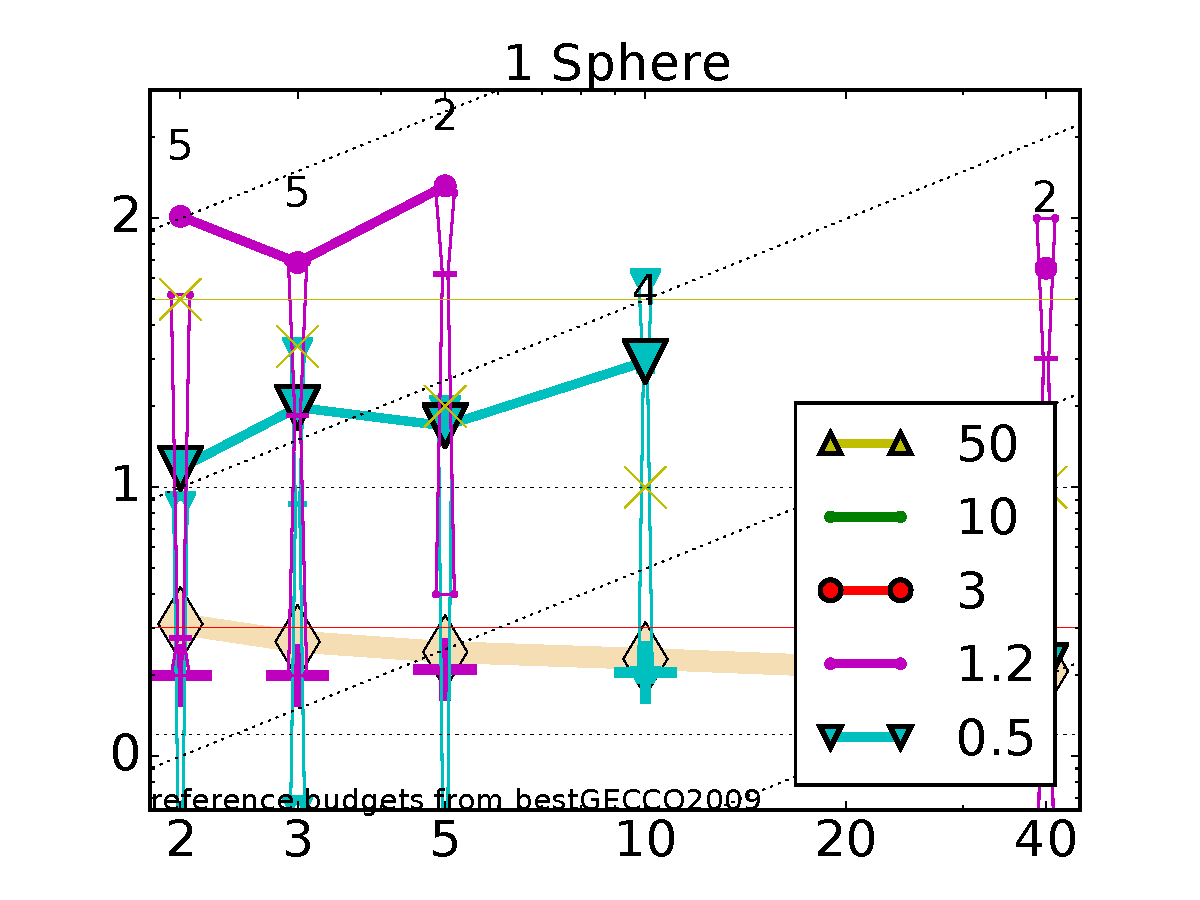
\includegraphics[width=0.268\textwidth]{ppfigdim_f001}&
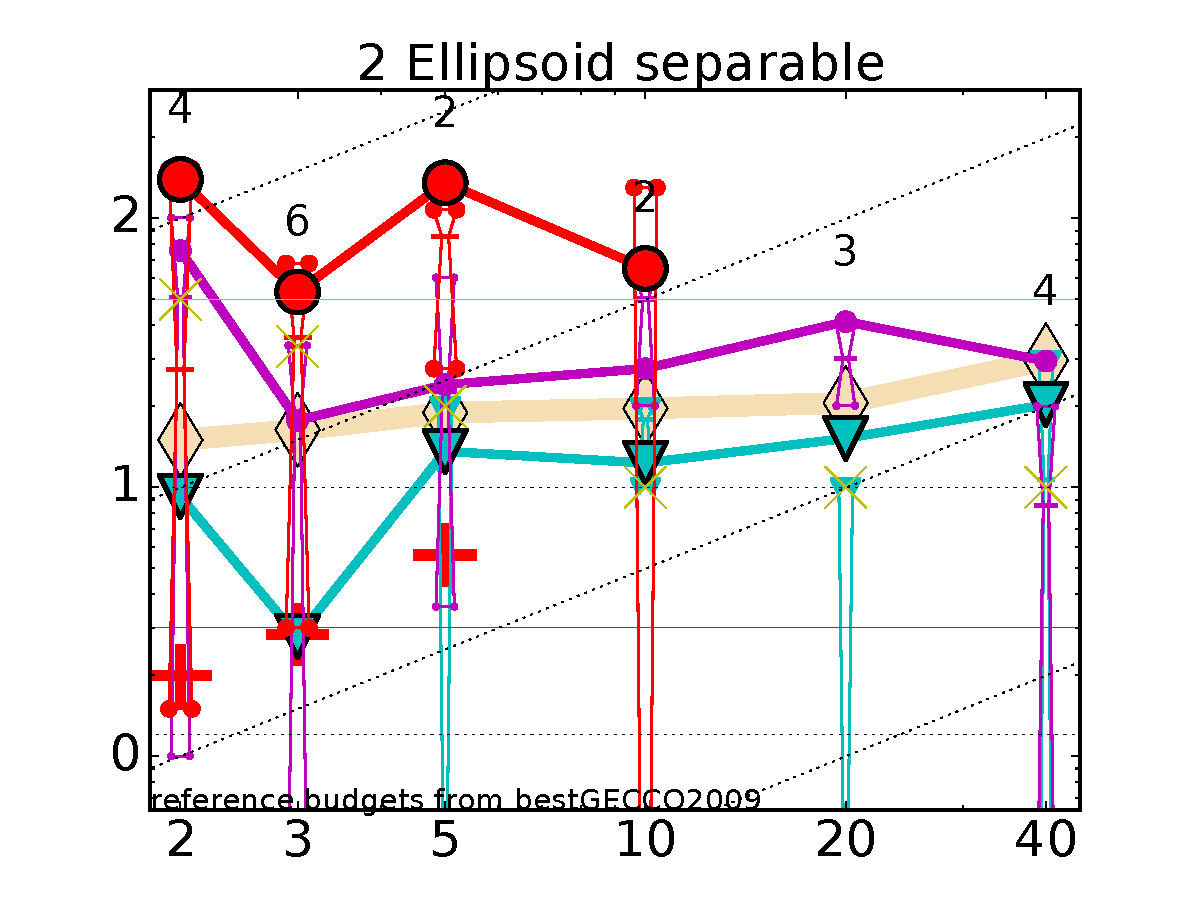
\includegraphics[width=0.268\textwidth]{ppfigdim_f002}&
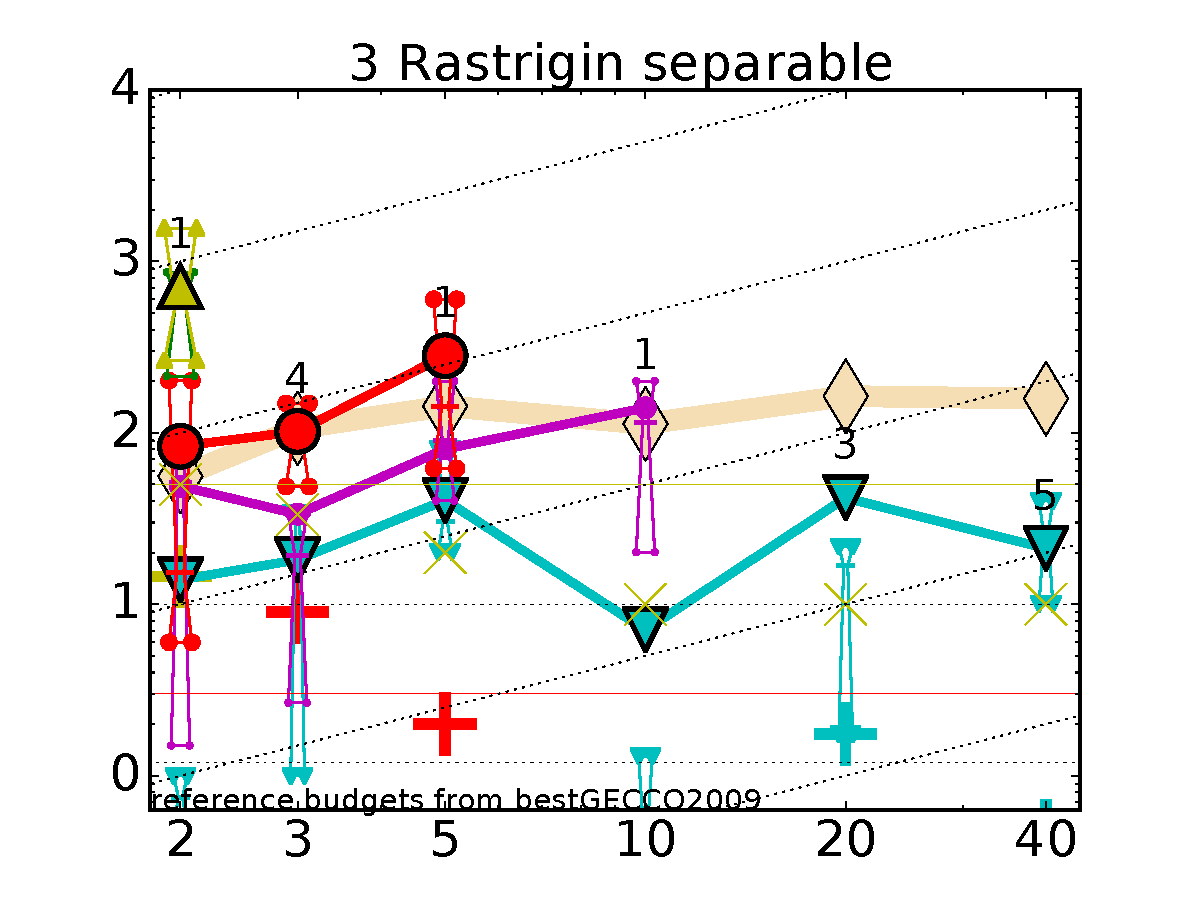
\includegraphics[width=0.268\textwidth]{ppfigdim_f003}&
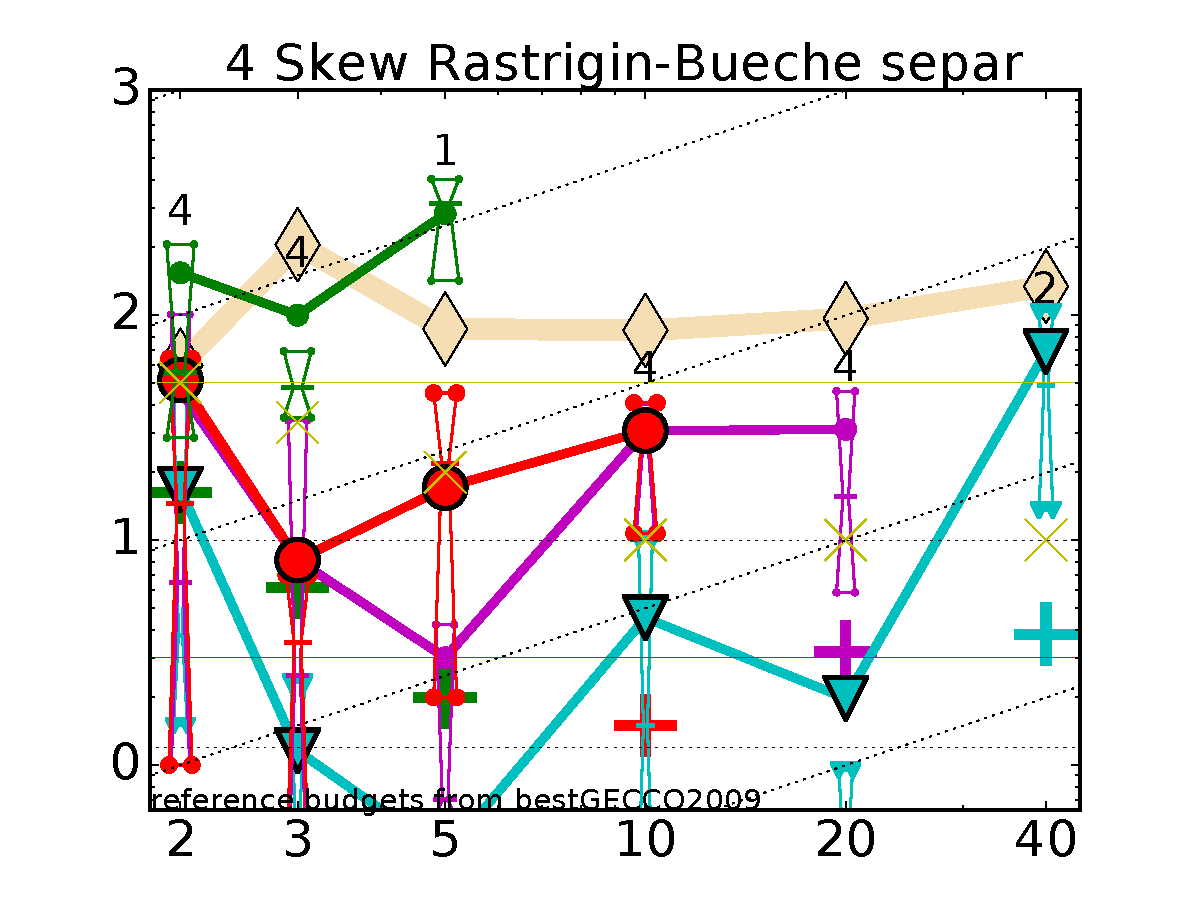
\includegraphics[width=0.268\textwidth]{ppfigdim_f004}\\[-2.2ex]
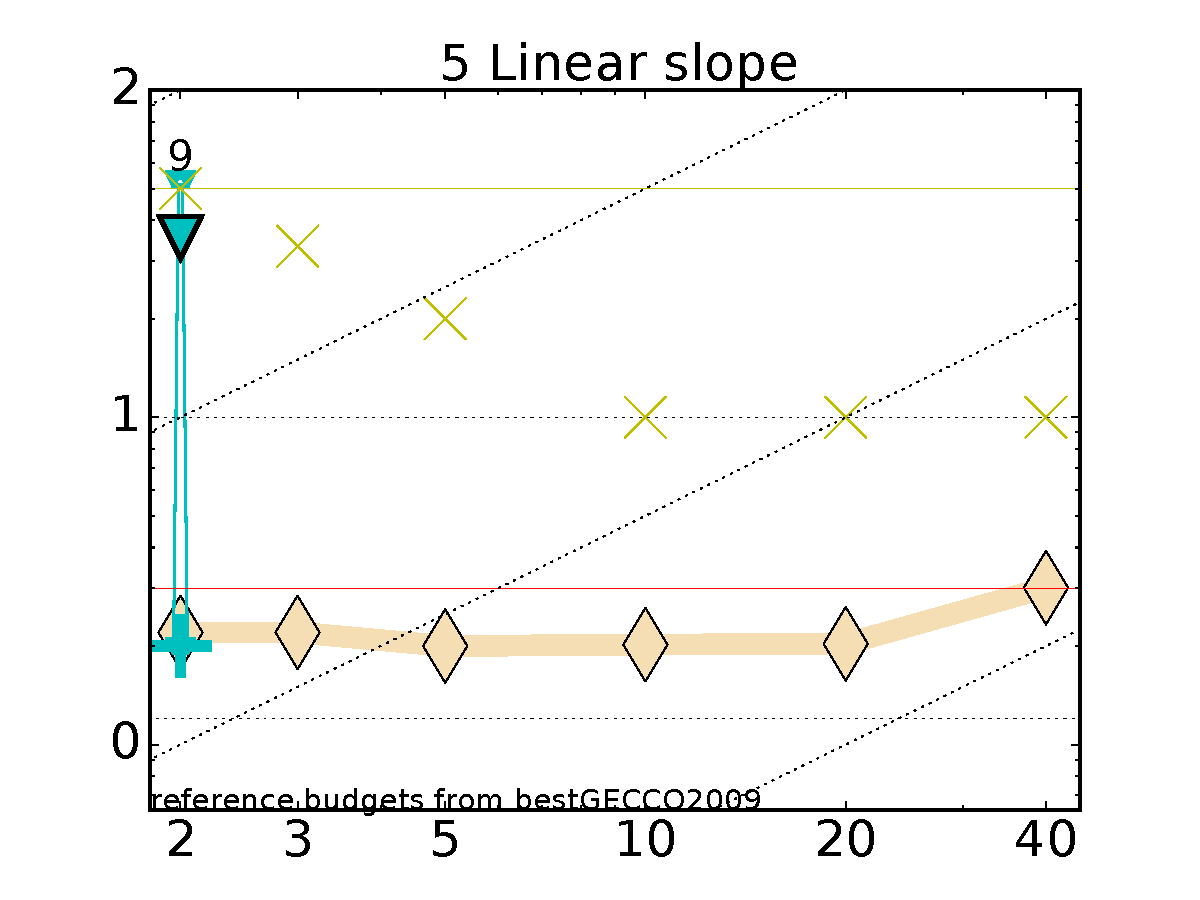
\includegraphics[width=0.268\textwidth]{ppfigdim_f005}&
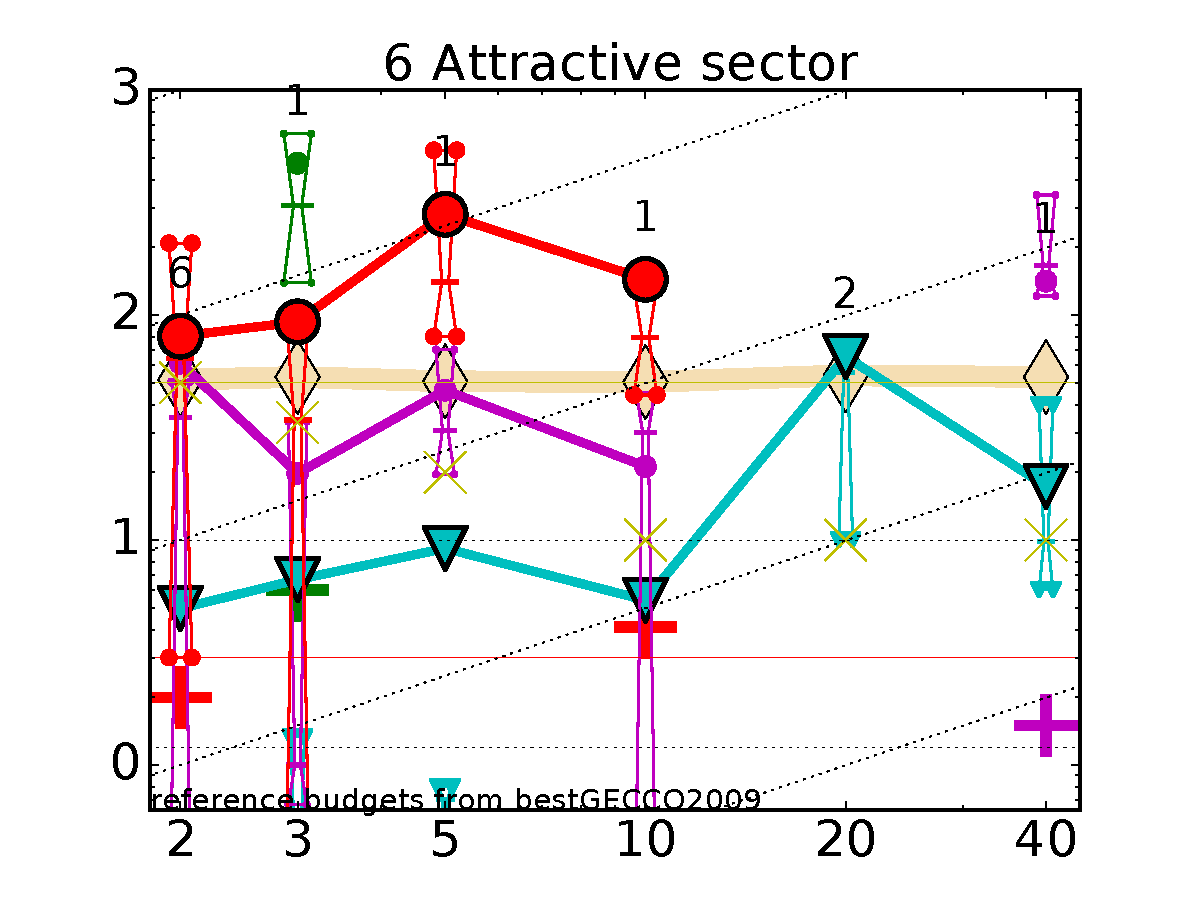
\includegraphics[width=0.268\textwidth]{ppfigdim_f006}&
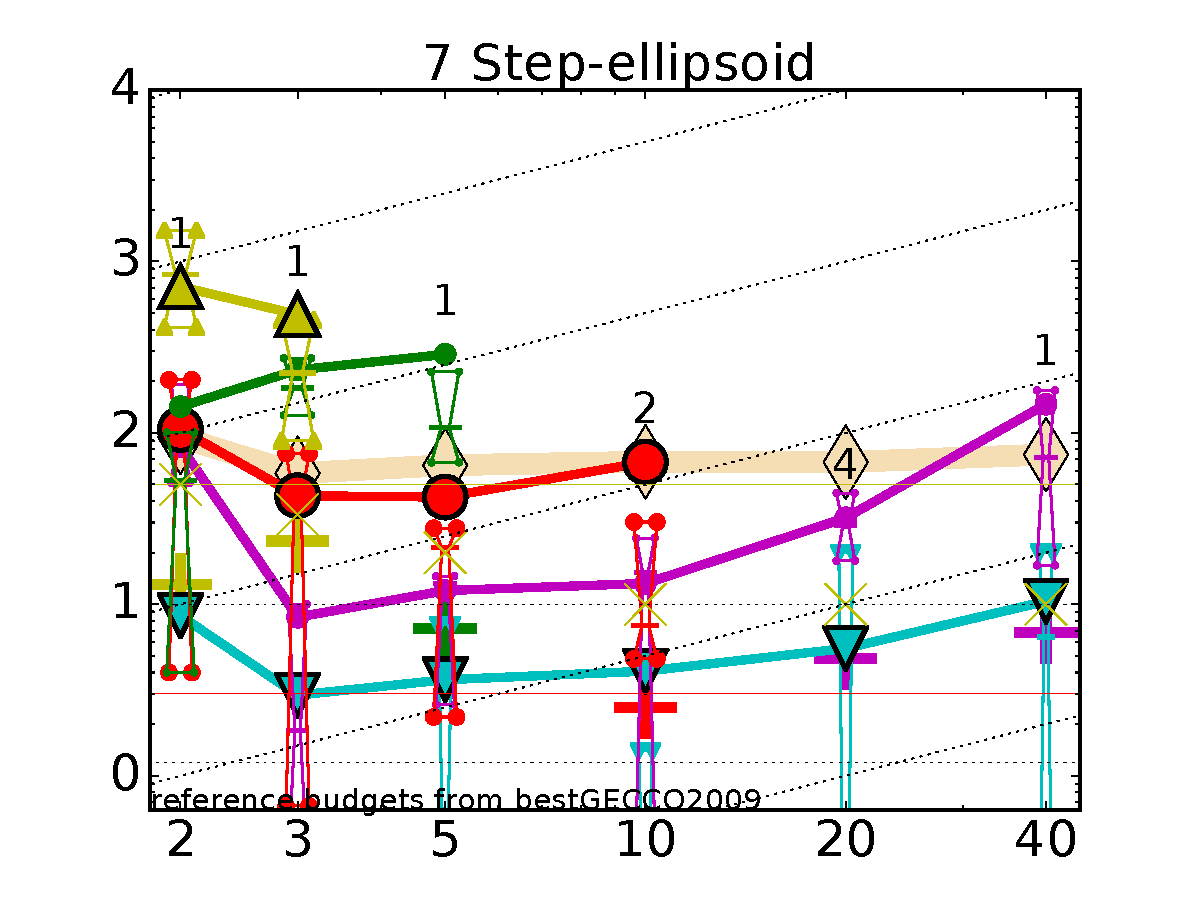
\includegraphics[width=0.268\textwidth]{ppfigdim_f007}&
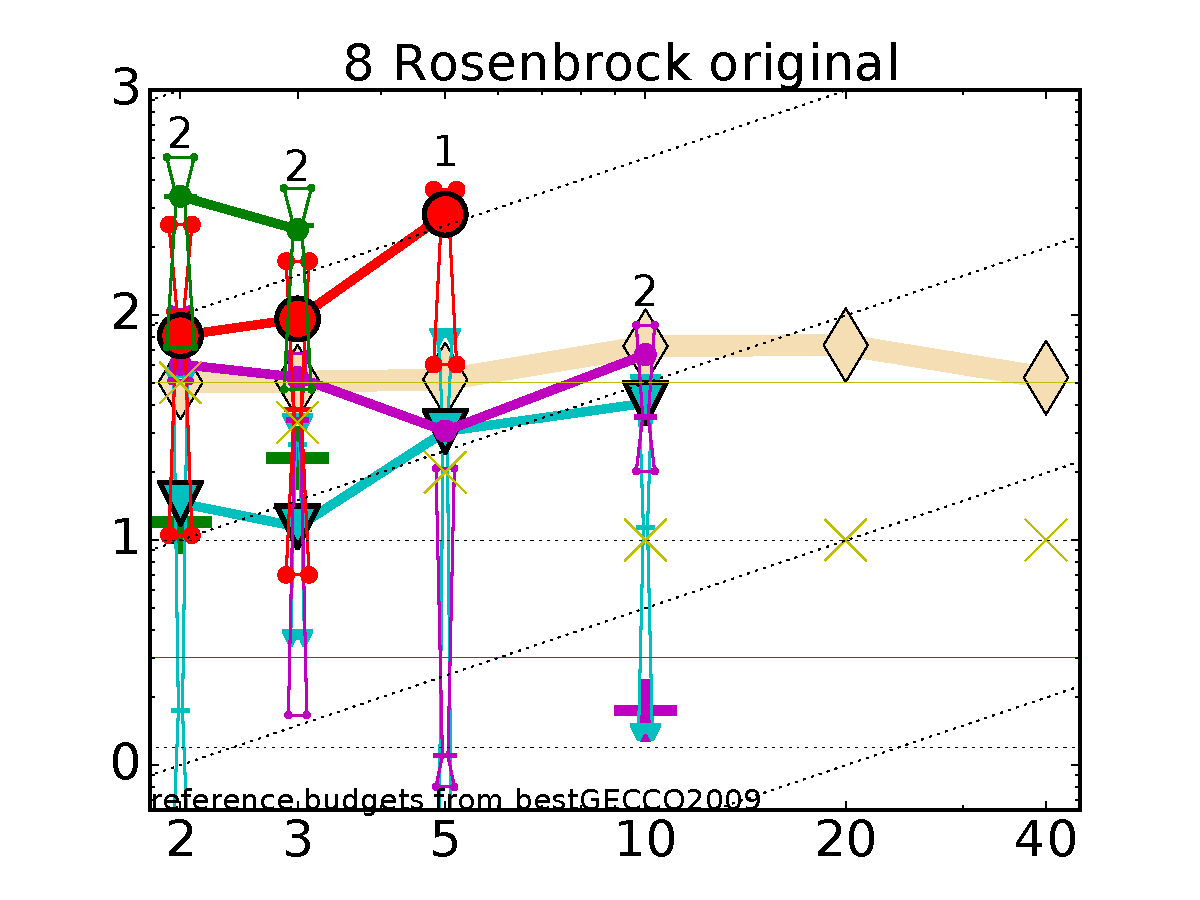
\includegraphics[width=0.268\textwidth]{ppfigdim_f008}\\[-2.2ex]
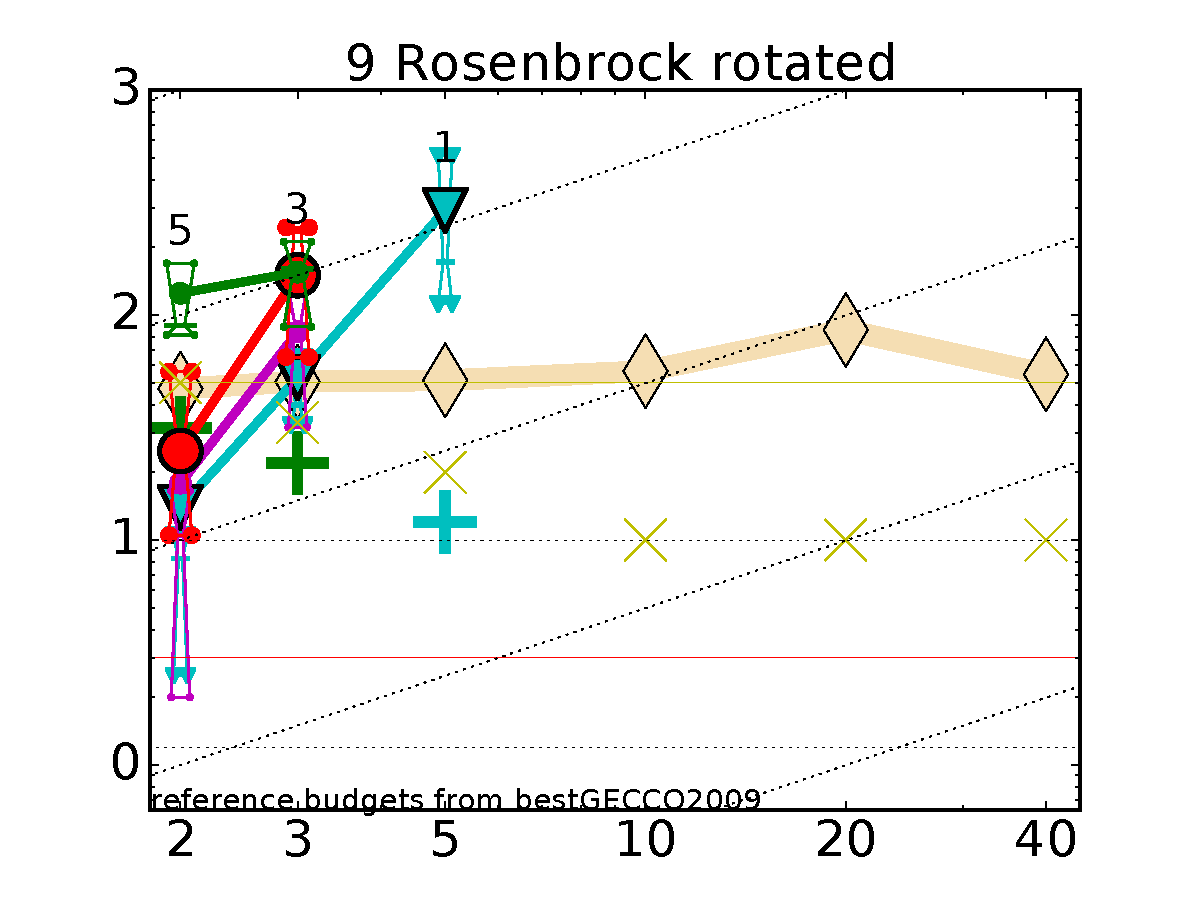
\includegraphics[width=0.268\textwidth]{ppfigdim_f009}&
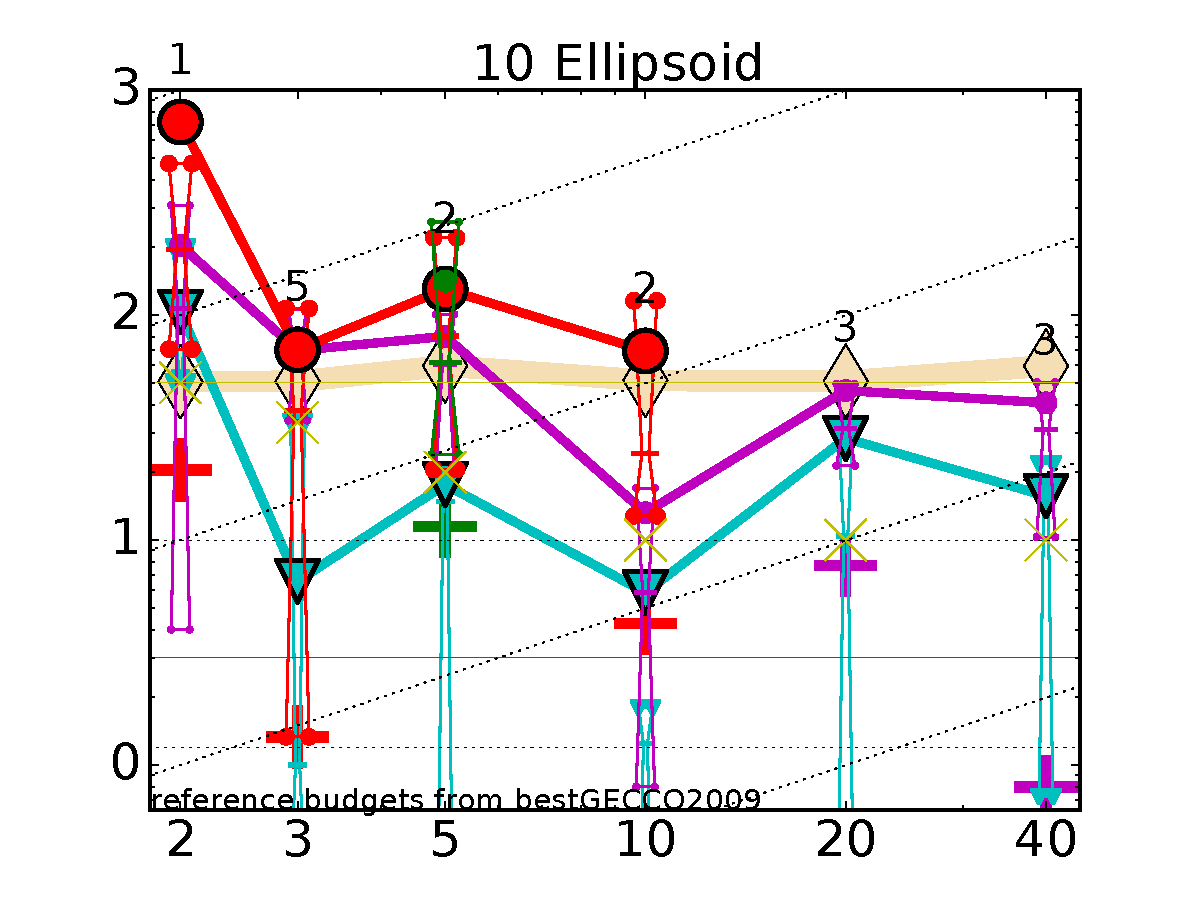
\includegraphics[width=0.268\textwidth]{ppfigdim_f010}&
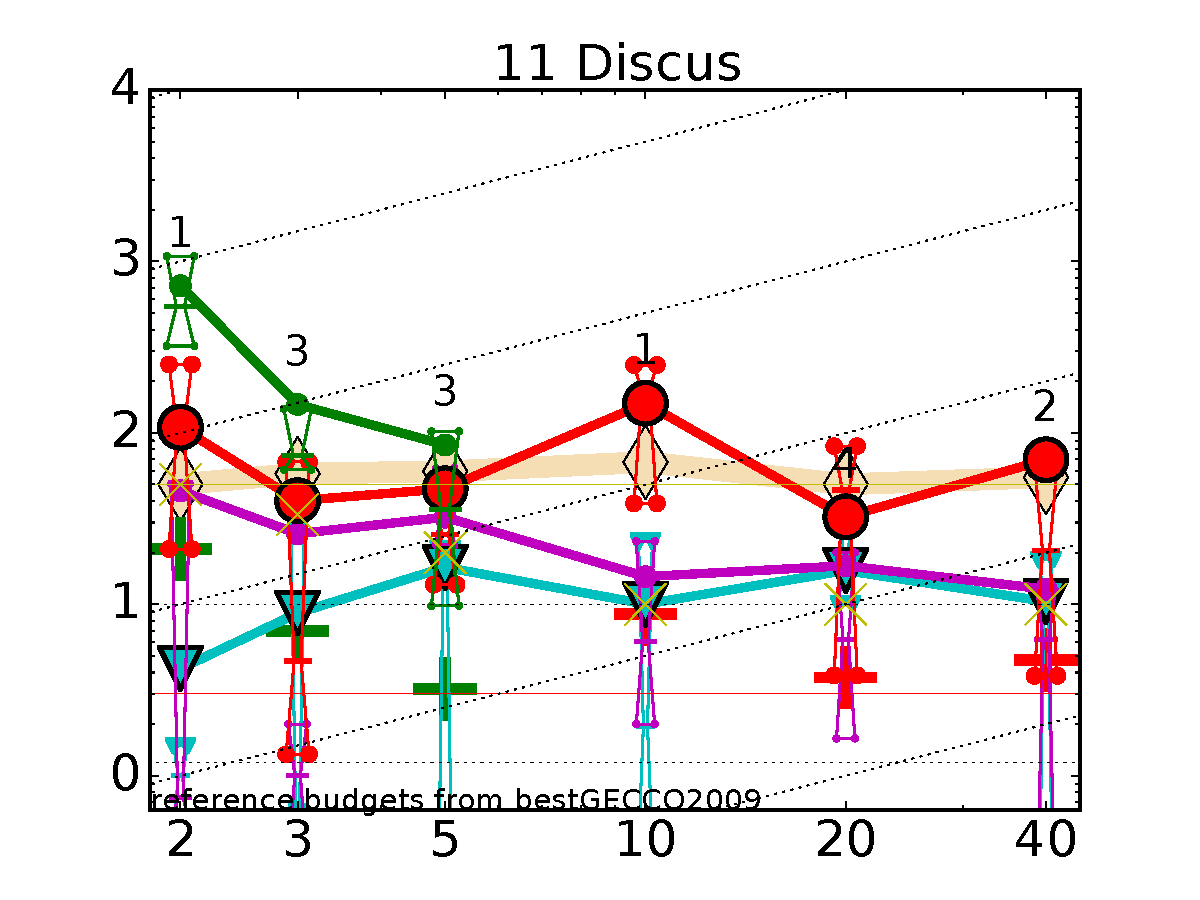
\includegraphics[width=0.268\textwidth]{ppfigdim_f011}&
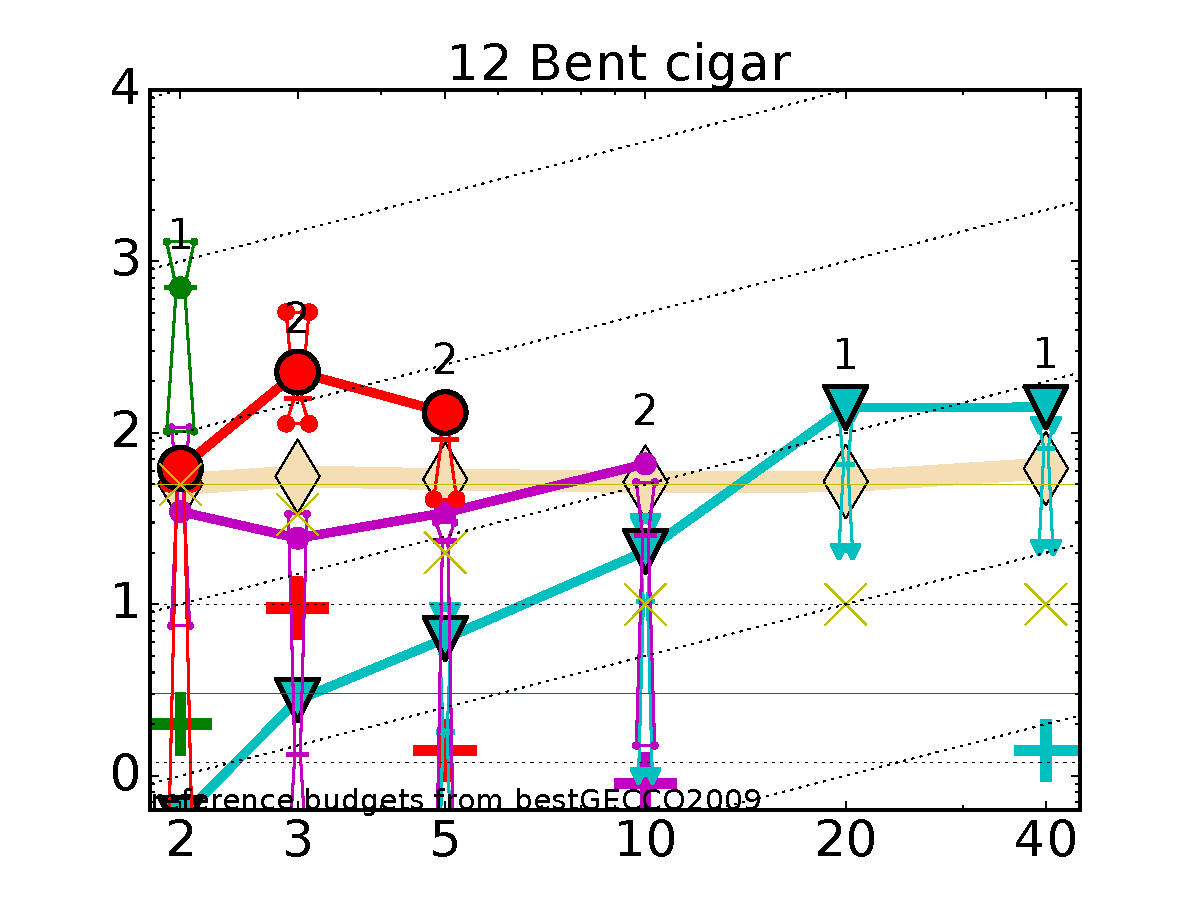
\includegraphics[width=0.268\textwidth]{ppfigdim_f012}\\[-2.2ex]
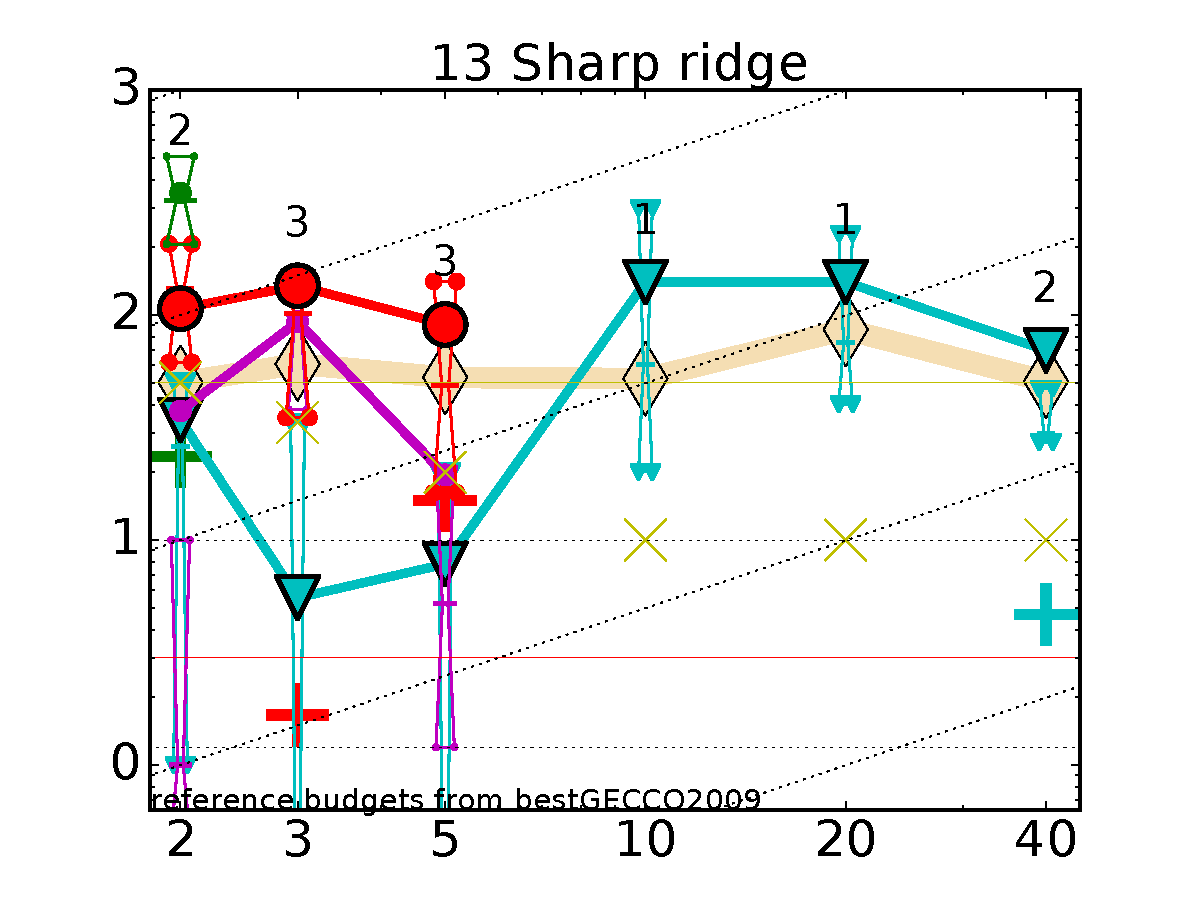
\includegraphics[width=0.268\textwidth]{ppfigdim_f013}&
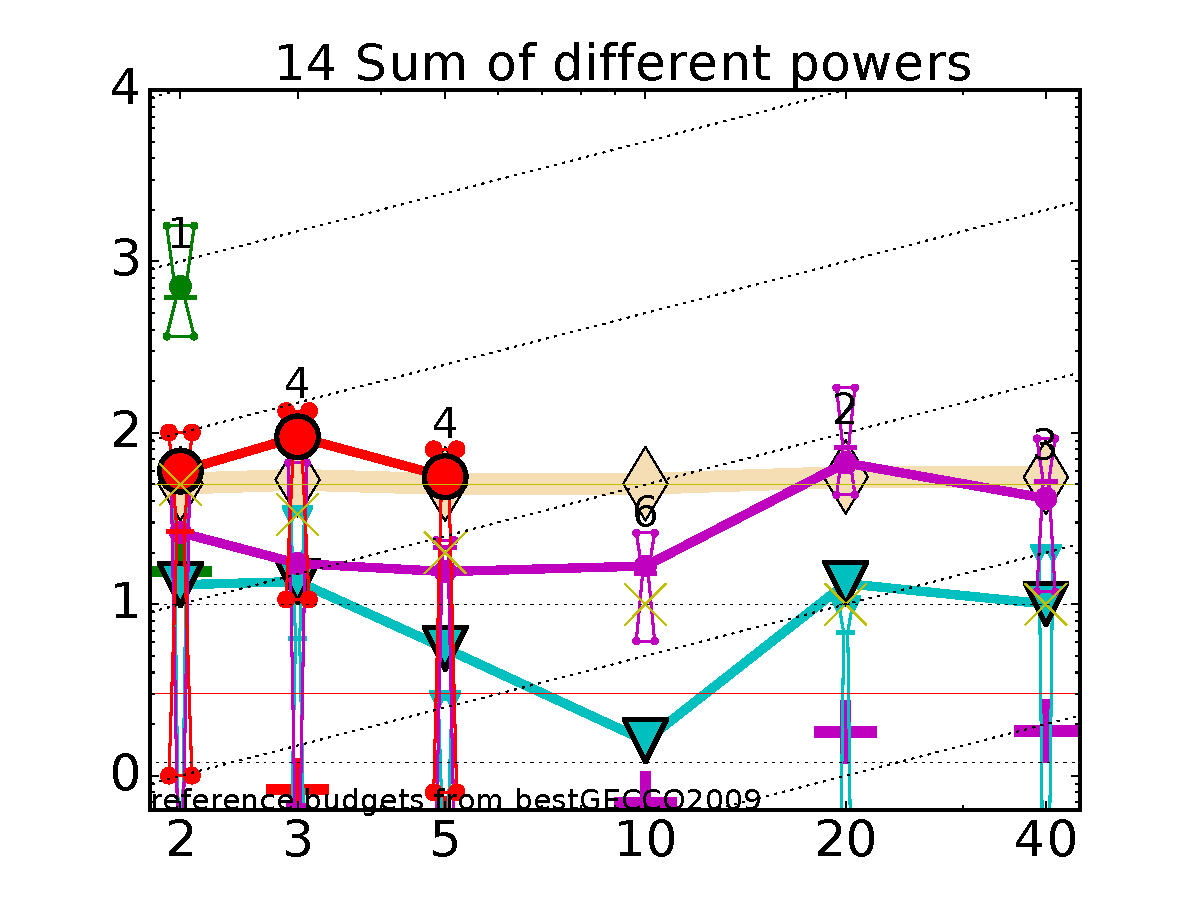
\includegraphics[width=0.268\textwidth]{ppfigdim_f014}&
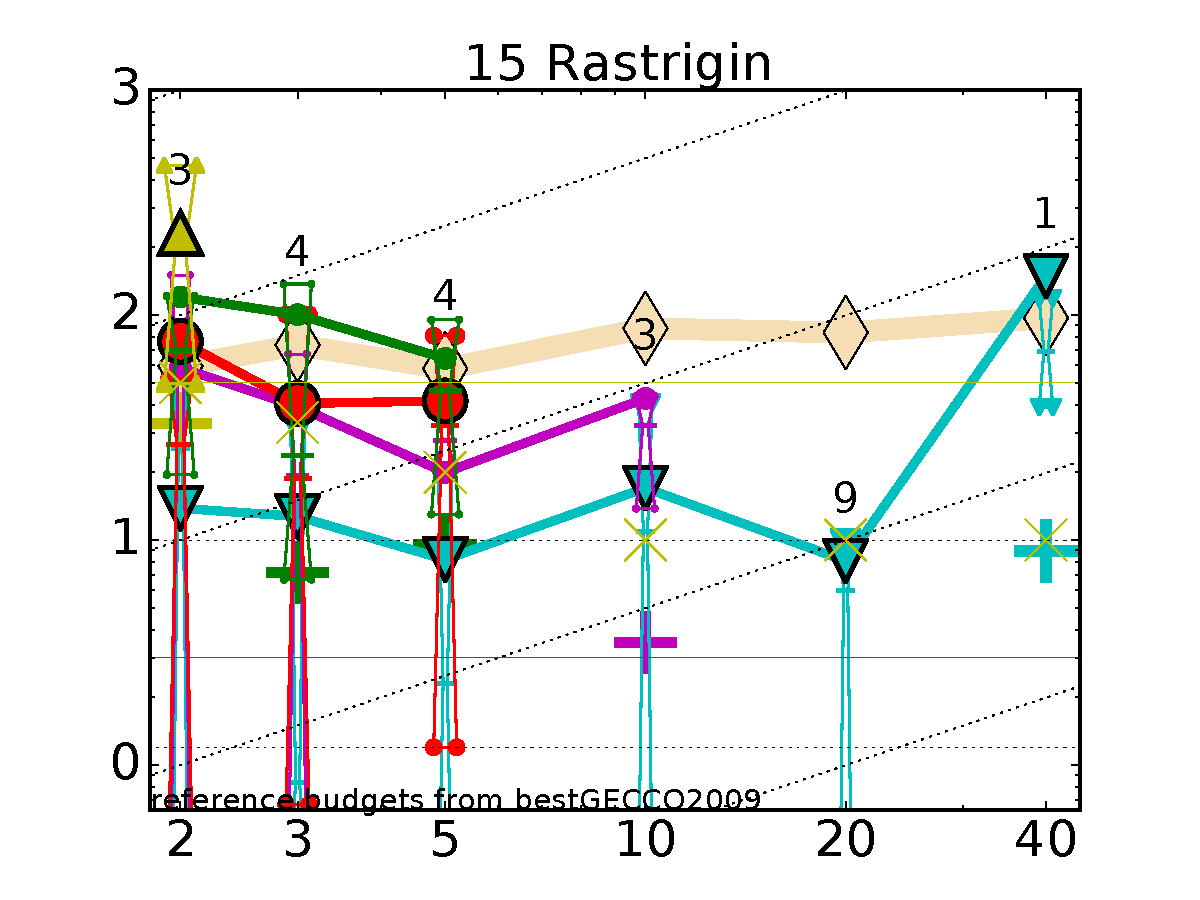
\includegraphics[width=0.268\textwidth]{ppfigdim_f015}&
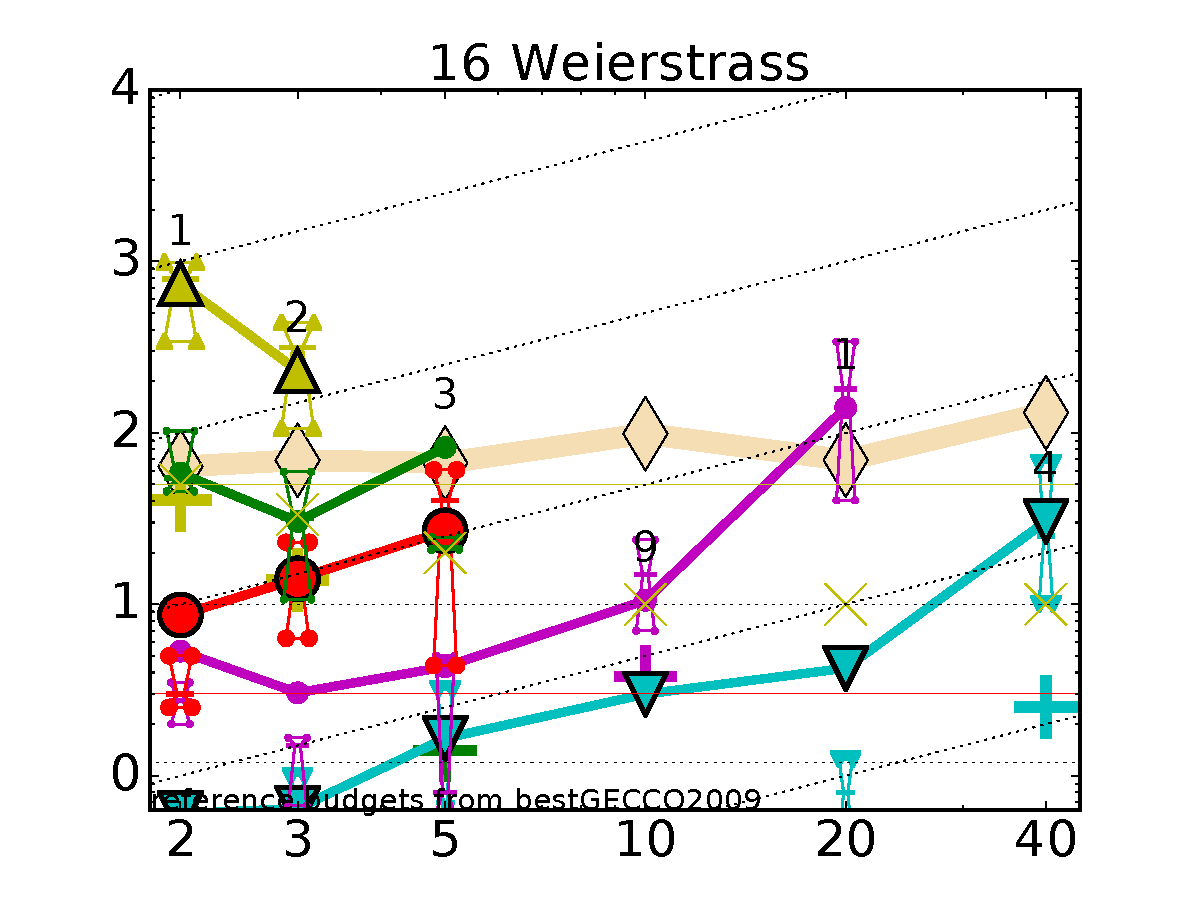
\includegraphics[width=0.268\textwidth]{ppfigdim_f016}\\[-2.2ex]
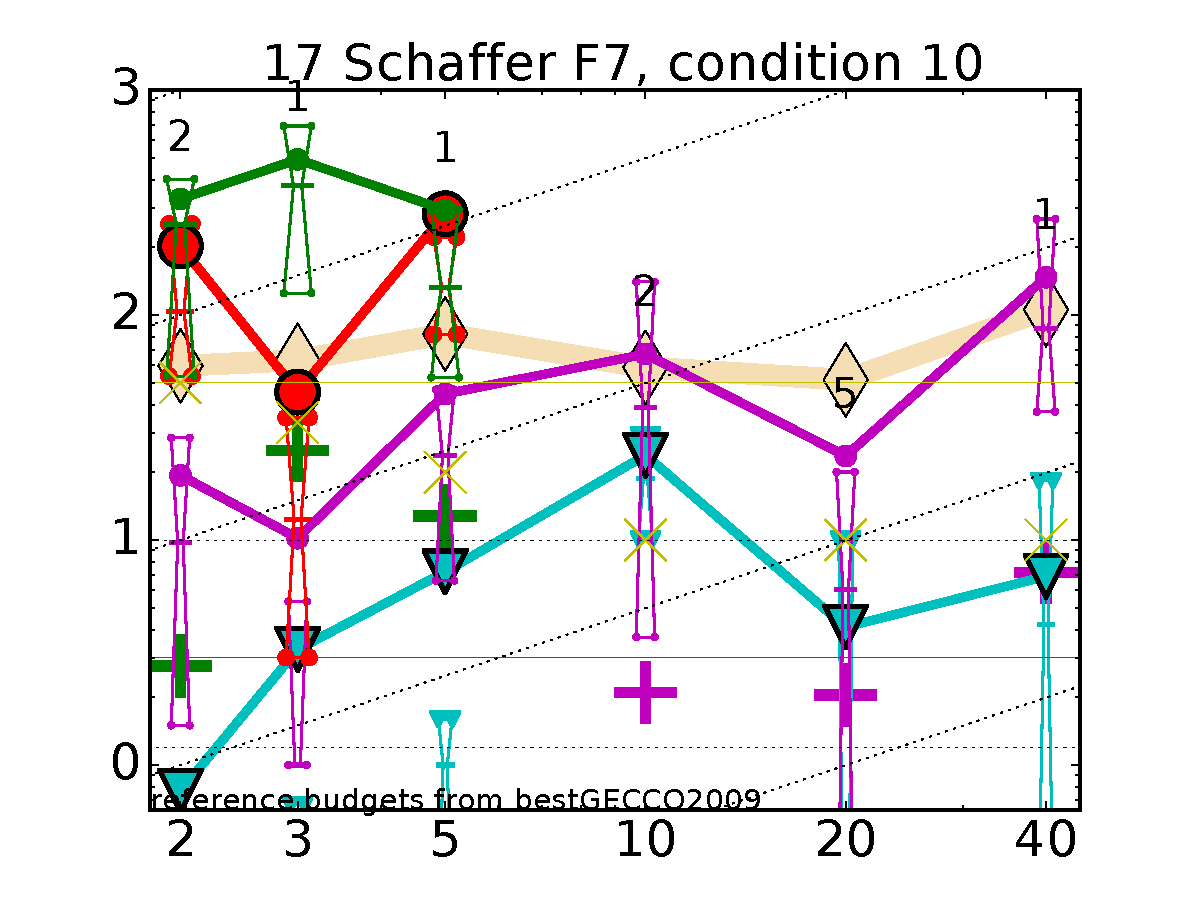
\includegraphics[width=0.268\textwidth]{ppfigdim_f017}&
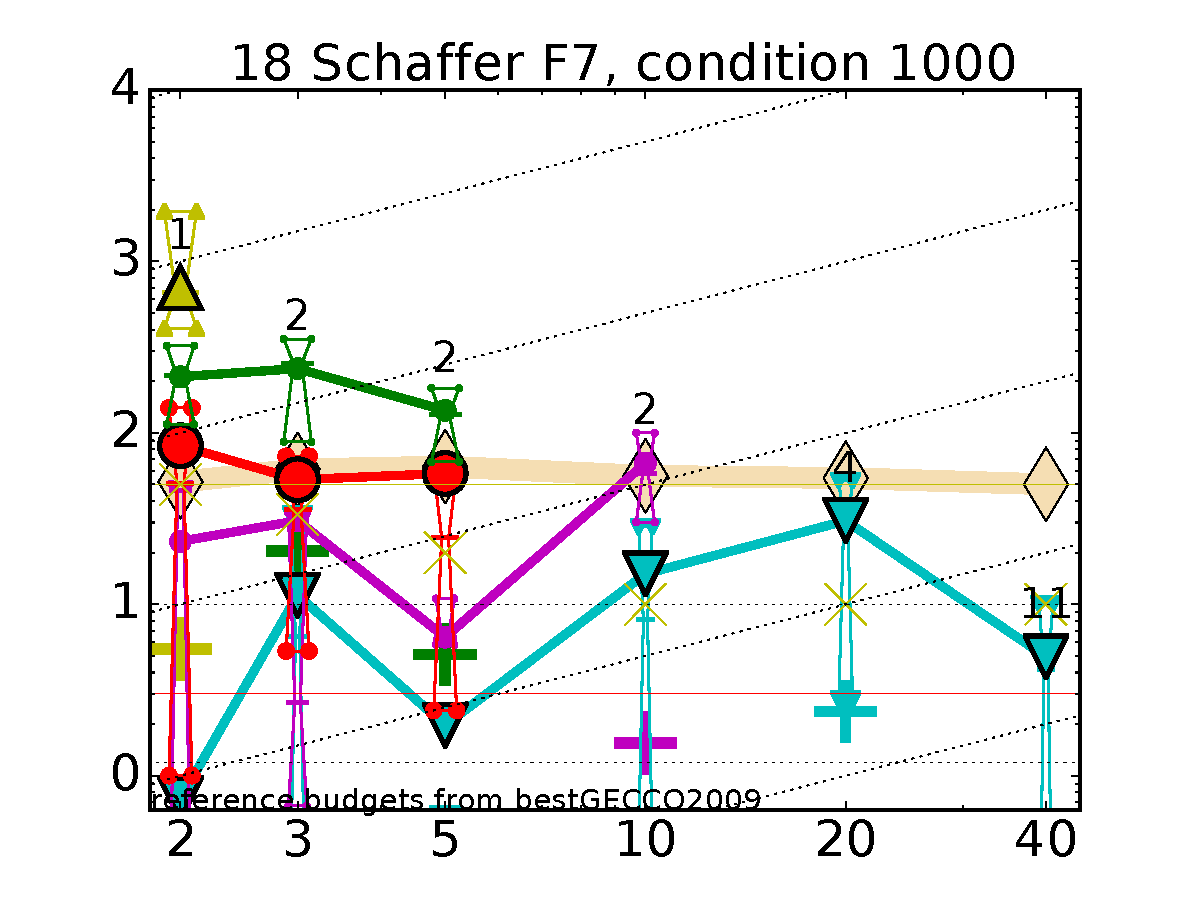
\includegraphics[width=0.268\textwidth]{ppfigdim_f018}&
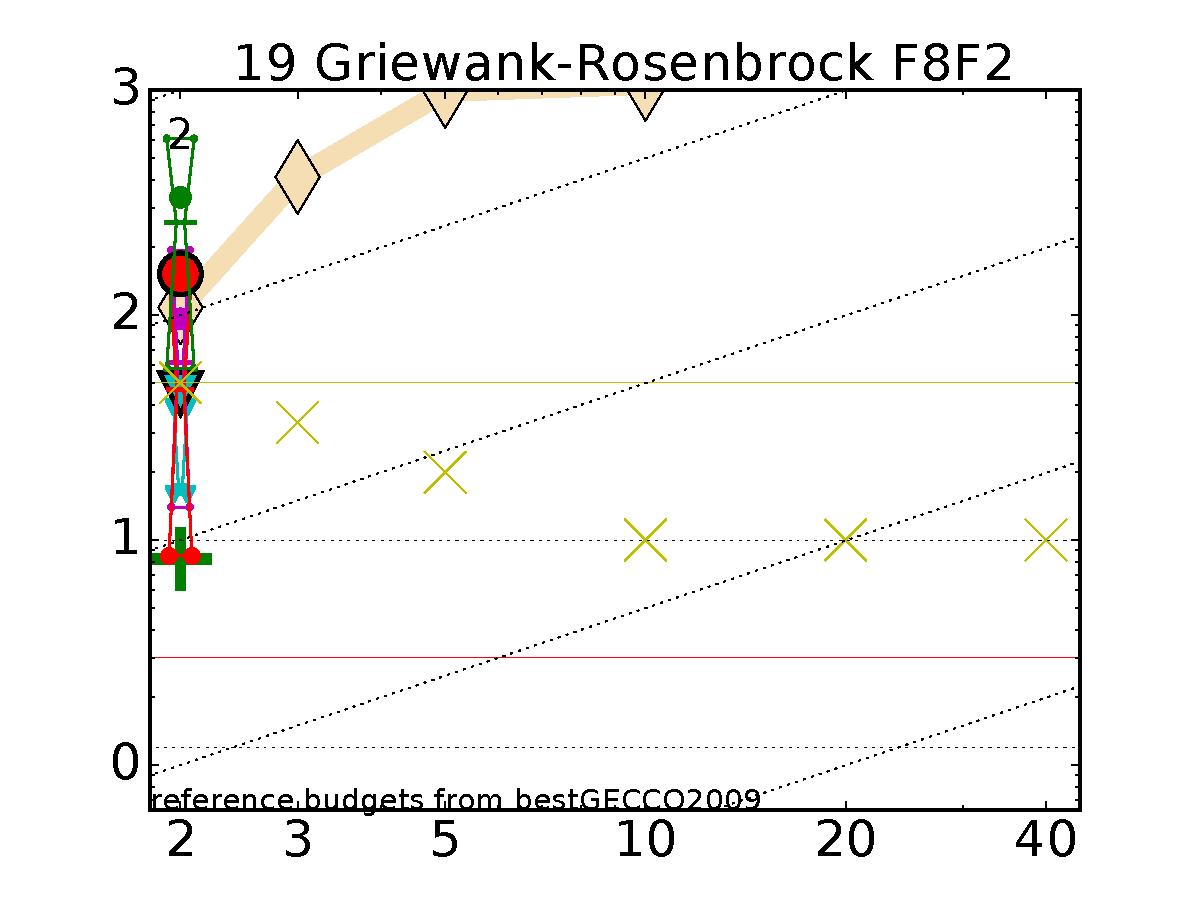
\includegraphics[width=0.268\textwidth]{ppfigdim_f019}&
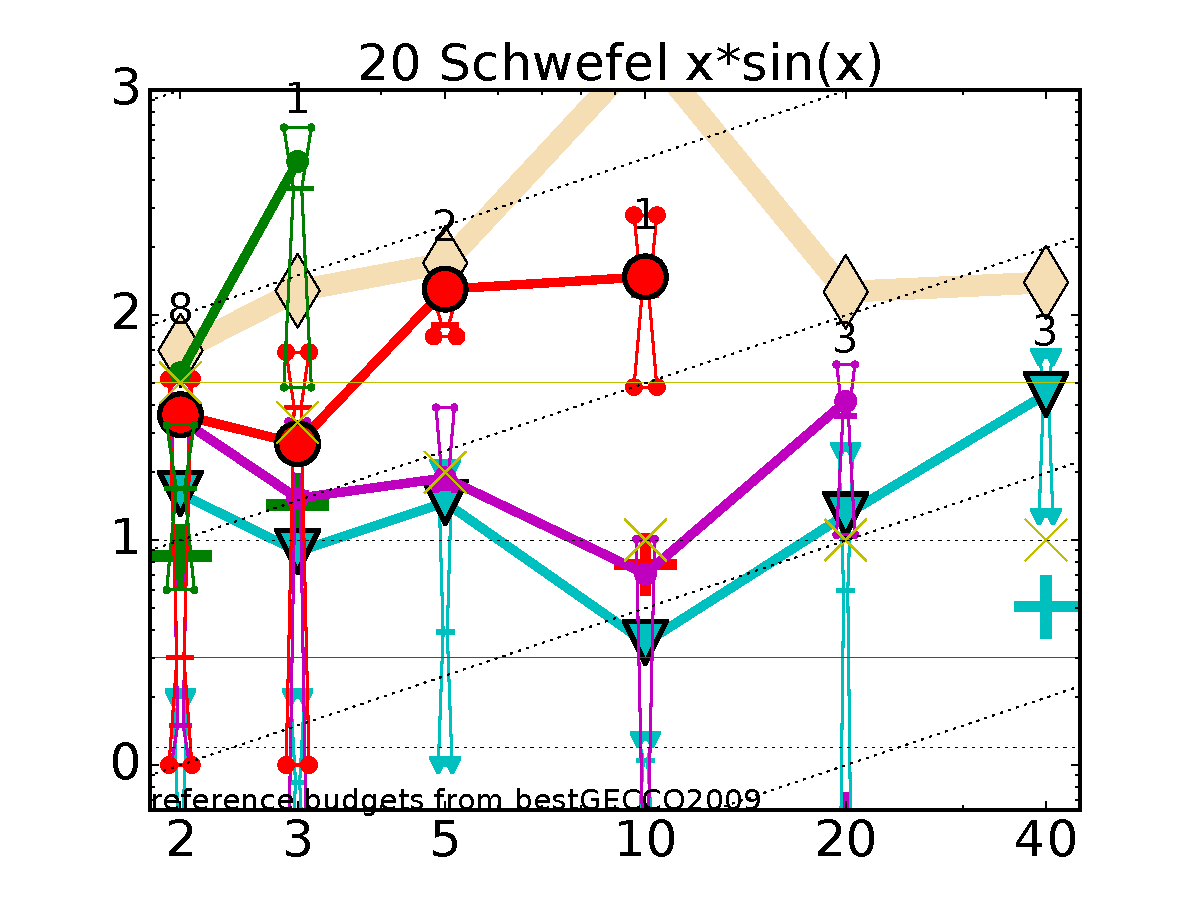
\includegraphics[width=0.268\textwidth]{ppfigdim_f020}\\[-2.2ex]
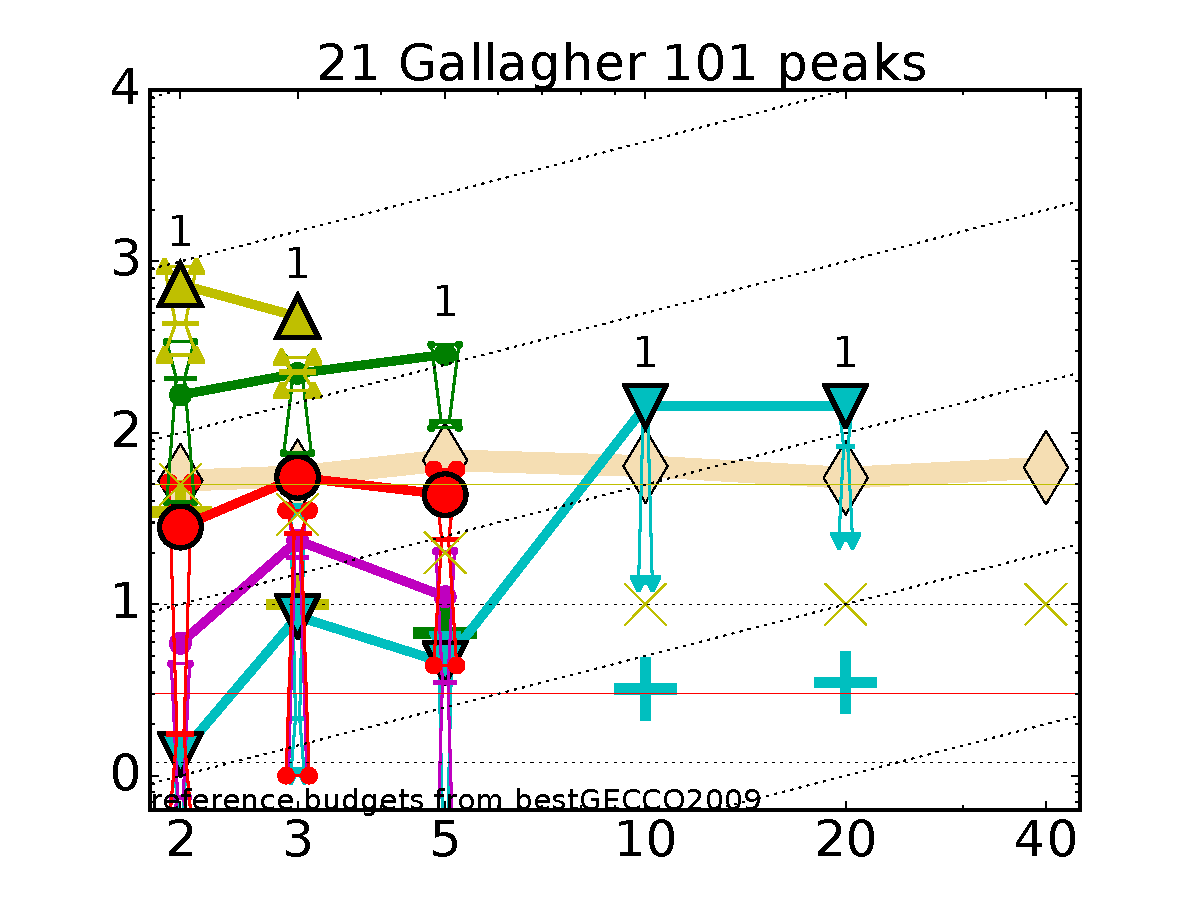
\includegraphics[width=0.268\textwidth]{ppfigdim_f021}&
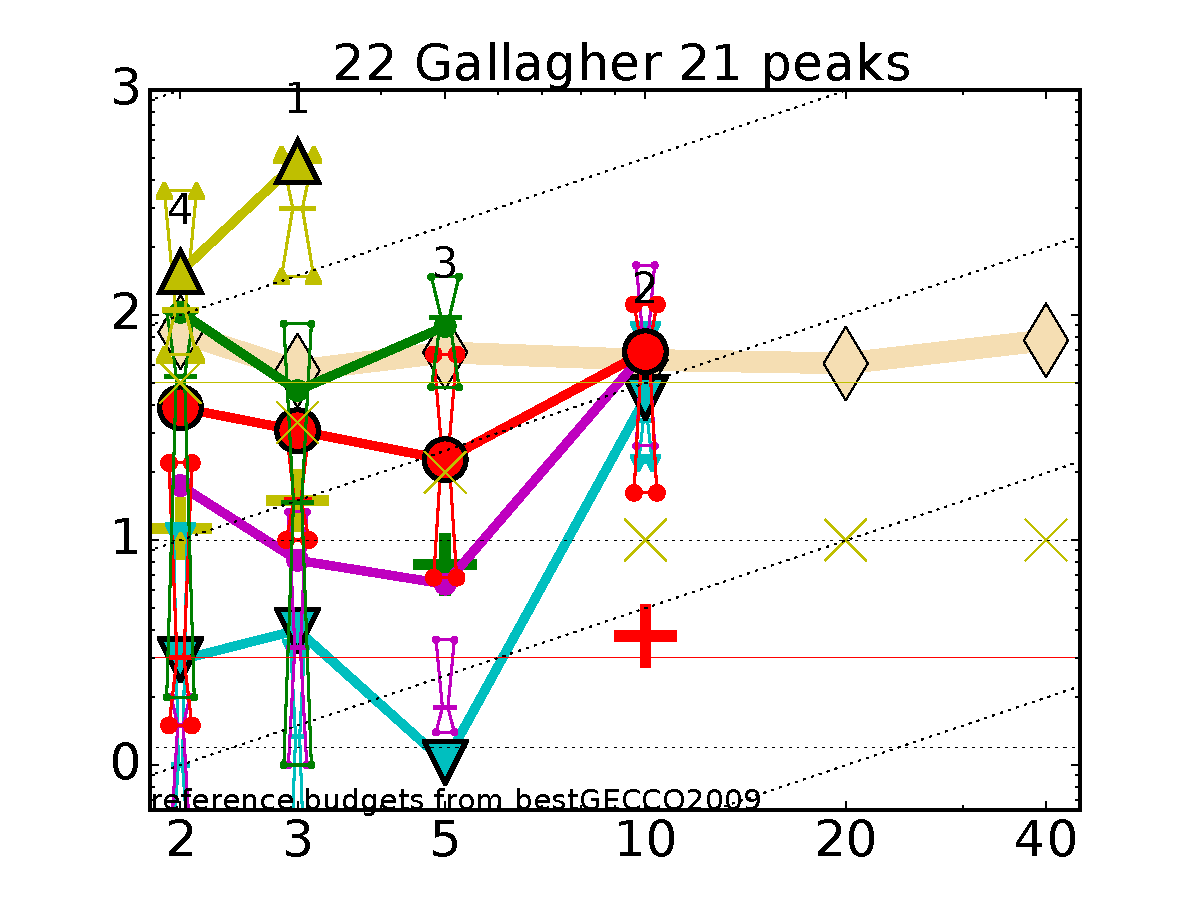
\includegraphics[width=0.268\textwidth]{ppfigdim_f022}&
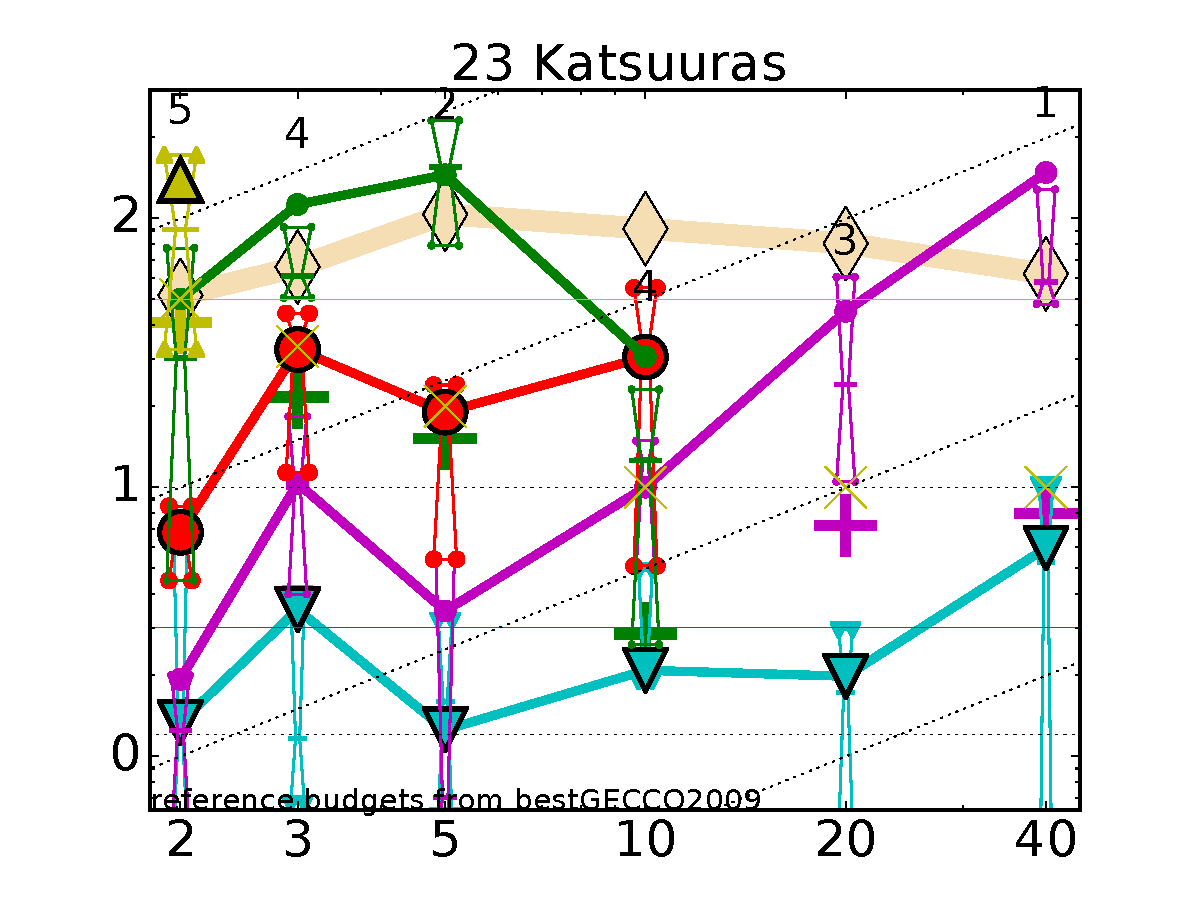
\includegraphics[width=0.268\textwidth]{ppfigdim_f023}&
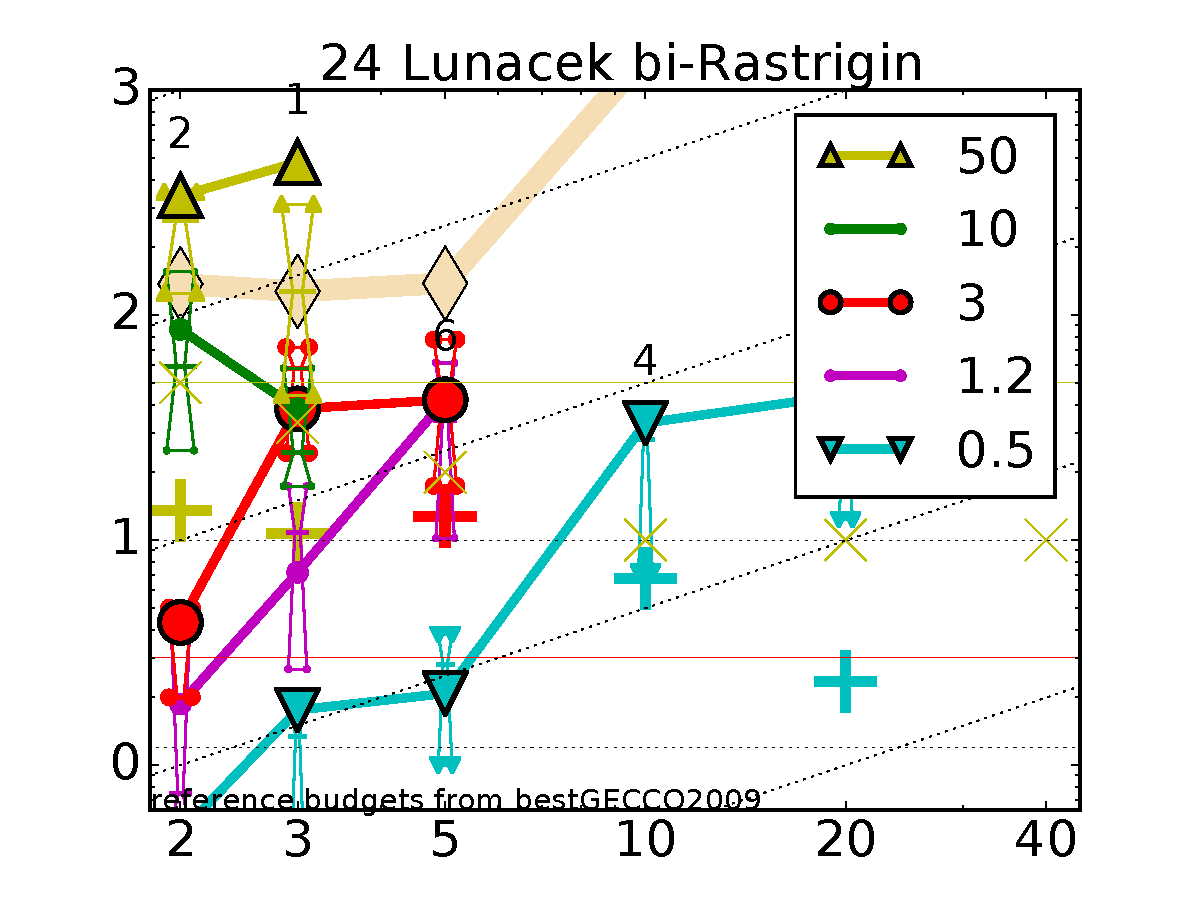
\includegraphics[width=0.268\textwidth]{ppfigdim_f024}
\end{tabular}
\vspace{-3ex}
 \caption{\label{fig:ERTgraphs}
 \bbobppfigdimlegend{$f_1$ and $f_{24}$}
 }
\end{figure*}

%%%%%%%%%%%%%%%%%%%%%%%%%%%%%%%%%%%%%%%%%%%%%%%%%%%%%%%%%%%%%%%%%%%%%%%%%%%%%%%
%%%%%%%%%%%%%%%%%%%%%%%%%%%%%%%%%%%%%%%%%%%%%%%%%%%%%%%%%%%%%%%%%%%%%%%%%%%%%%%
 
% Table showing the expected running time (ERT in number of function
% evaluations) divided by the best ERT measured during BBOB-2009 (given in the
% first row of each cell) for functions $f_1$--$f_{24}$.

%%%%%%%%%%%%%%%%%%%%%%%%%%%%%%%%%%%%%%%%%%%%%%%%%%%%%%%%%%%%%%%%%%%%%%%%%%%%%%%

\begin{table*}
\centering {\tiny
\parbox{0.499\textwidth}{\centering
   {\small 5-D}\\
   \input{\bbobdatapath\algfolder pptable_05D_noiselessall}}%
\parbox{0.499\textwidth}{\centering
   {\small 20-D}\\
   \input{\bbobdatapath\algfolder pptable_20D_noiselessall}}}\vspace{1em}
\caption[Table of ERTs]{\label{tab:ERTs}\bbobpptablecaption{}
}
\end{table*}
%%%%%%%%%%%%%%%%%%%%%%%%%%%%%%%%%%%%%%%%%%%%%%%%%%%%%%%%%%%%%%%%%%%%%%%%%%%%%%%
%%%%%%%%%%%%%%%%%%%%%%%%%%%%%%%%%%%%%%%%%%%%%%%%%%%%%%%%%%%%%%%%%%%%%%%%%%%%%%%


%%%%%%%%%%%%%%%%%%%%%%%%%%%%%%%%%%%%%%%%%%%%%%%%%%%%%%%%%%%%%%%%%%%%%%%%%%%%%%%
%%%%%%%%%%%%%%%%%%%%%%%%%%%%%%%%%%%%%%%%%%%%%%%%%%%%%%%%%%%%%%%%%%%%%%%%%%%%%%%

% Empirical cumulative distribution functions (ECDFs) per function group.

%%%%%%%%%%%%%%%%%%%%%%%%%%%%%%%%%%%%%%%%%%%%%%%%%%%%%%%%%%%%%%%%%%%%%%%%%%%%%%%
\newcommand{\rot}[2][2.5]{
  \hspace*{-3.5\baselineskip}%
  \begin{rotate}{90}\hspace{#1em}#2
  \end{rotate}}
\begin{figure*}
\begin{tabular}{l@{\hspace*{-0.025\textwidth}}l@{\hspace*{-0.00\textwidth}}|l@{\hspace*{-0.025\textwidth}}l}
\multicolumn{2}{c}{$D=5$} & \multicolumn{2}{c}{$D=20$}\\[-0.5ex]
\rot{separable fcts}
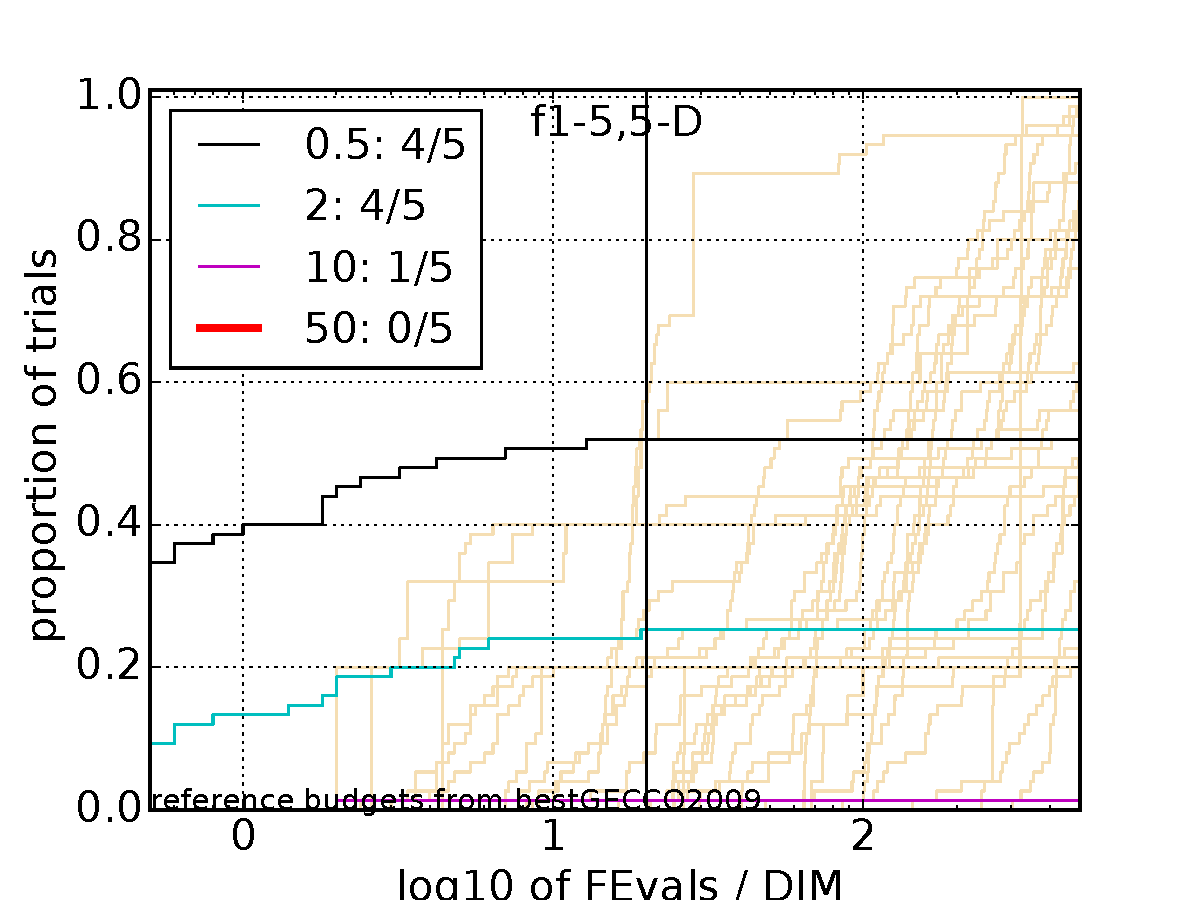
\includegraphics[width=0.268\textwidth,trim=0 0 0 13mm, clip]{pprldistr_05D_separ} &
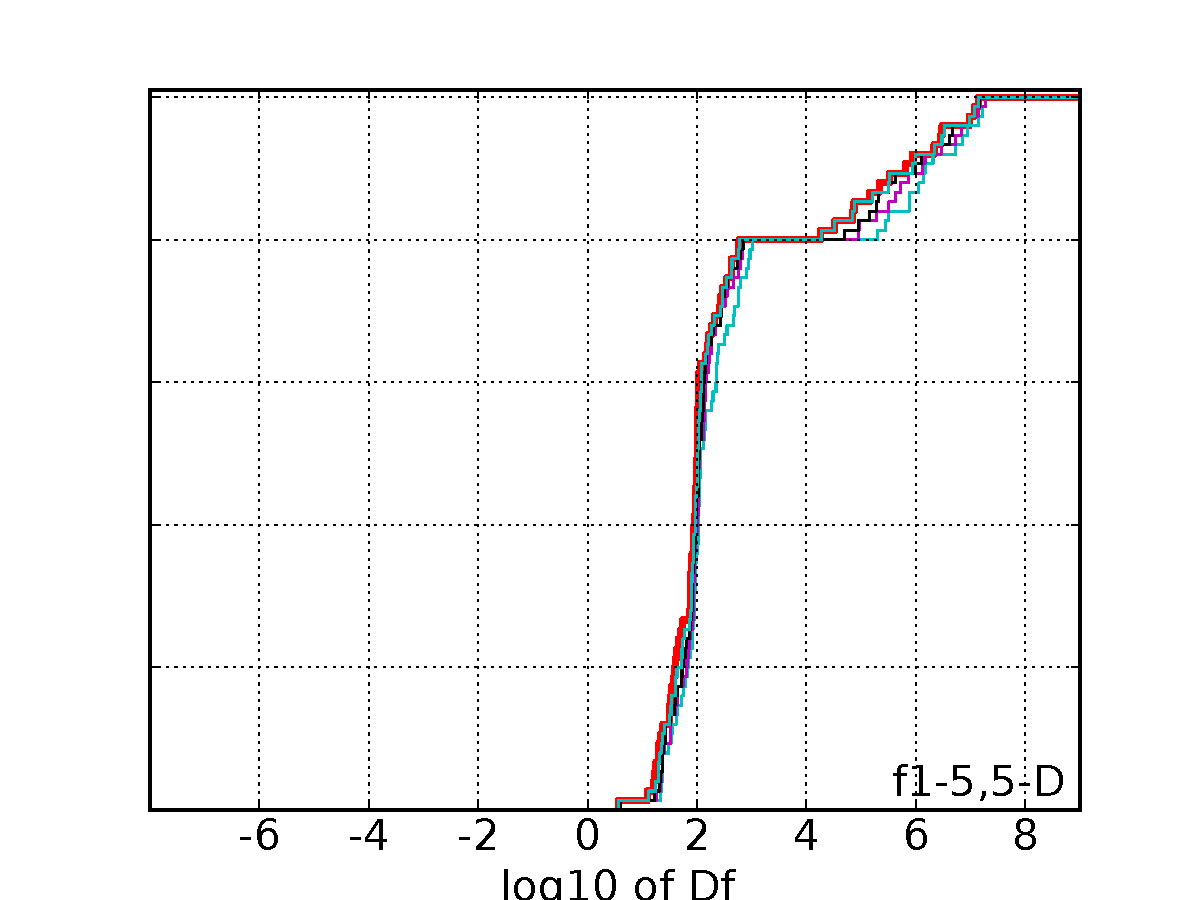
\includegraphics[width=0.2362\textwidth,trim=2.40cm 0 0 13mm, clip]{ppfvdistr_05D_separ} &
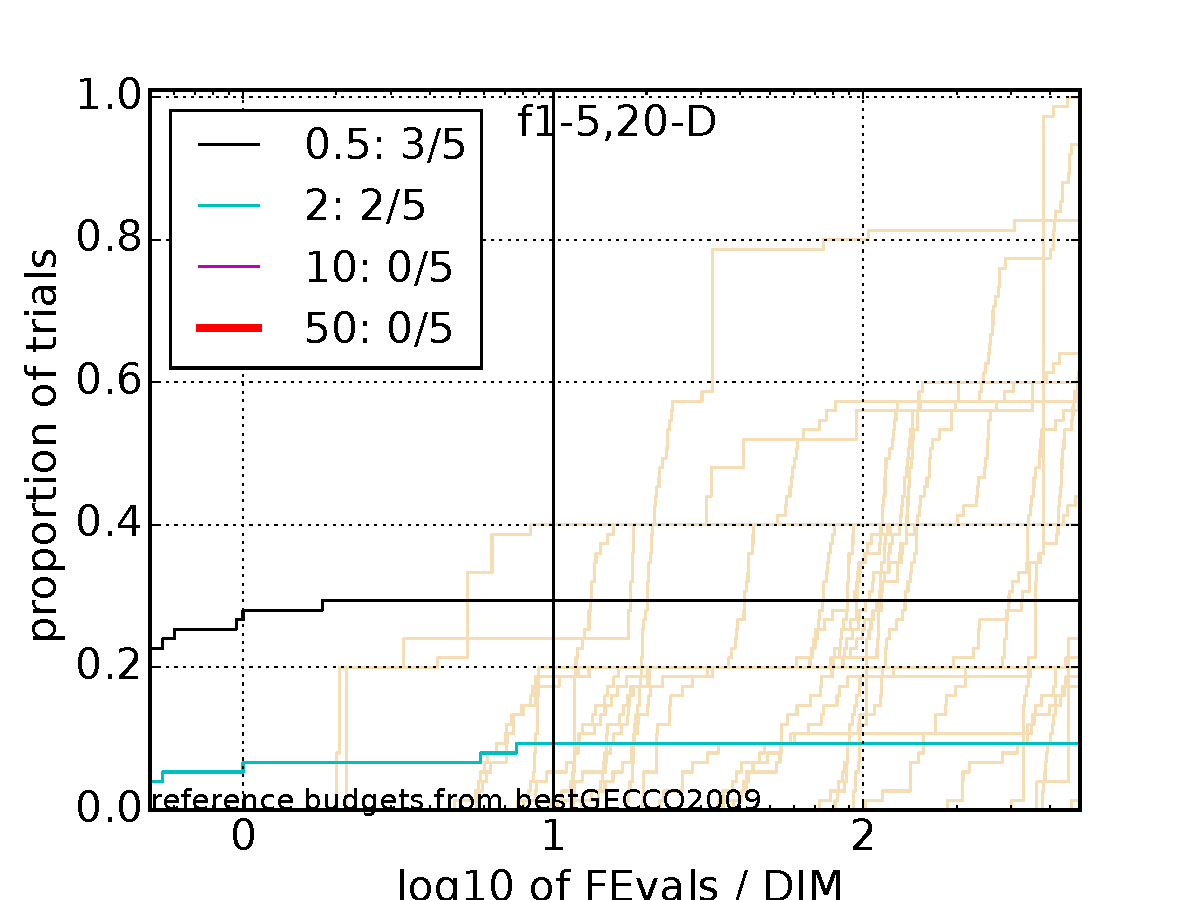
\includegraphics[width=0.268\textwidth,trim=0 0 0 13mm, clip]{pprldistr_20D_separ} &
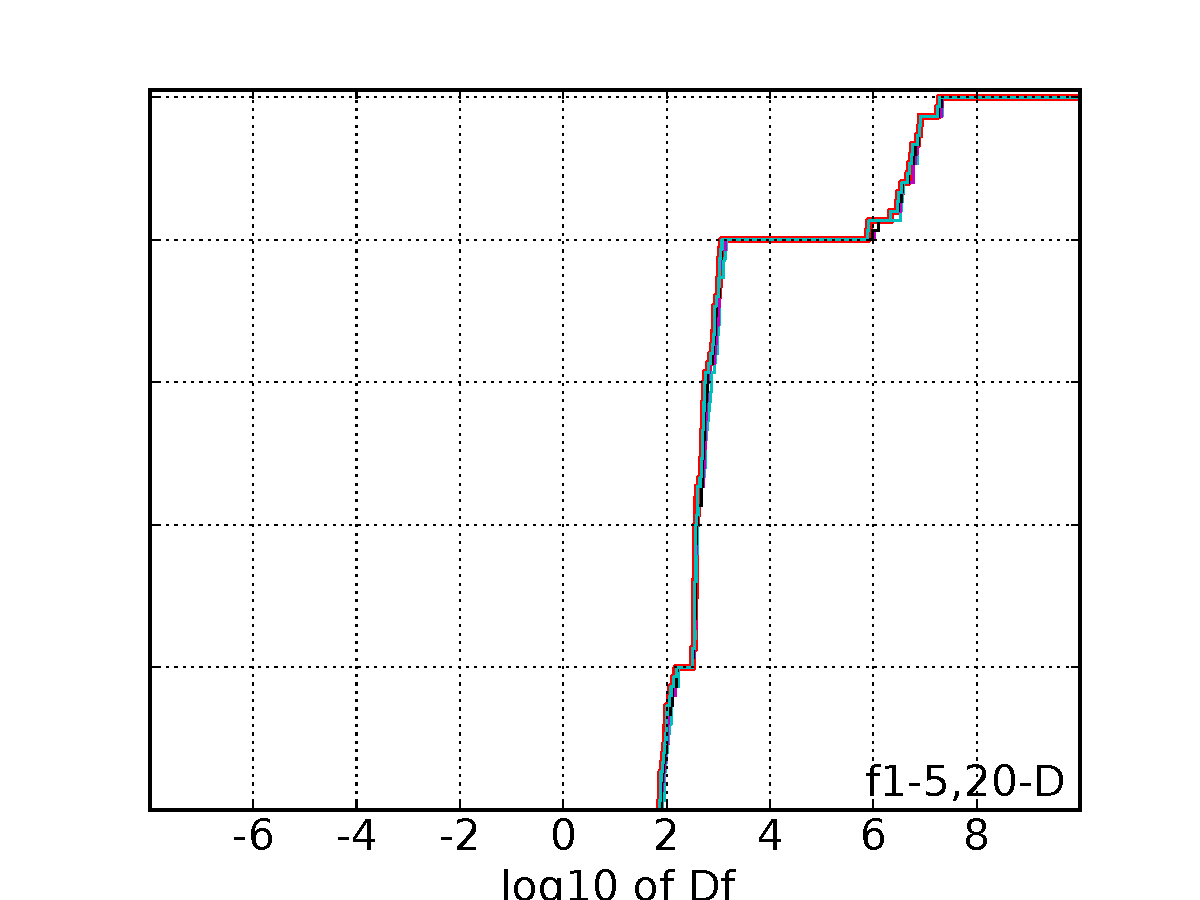
\includegraphics[width=0.2362\textwidth,trim=2.40cm 0 0 13mm, clip]{ppfvdistr_20D_separ} \\[-2ex]
\rot[1]{misc.\ moderate fcts}
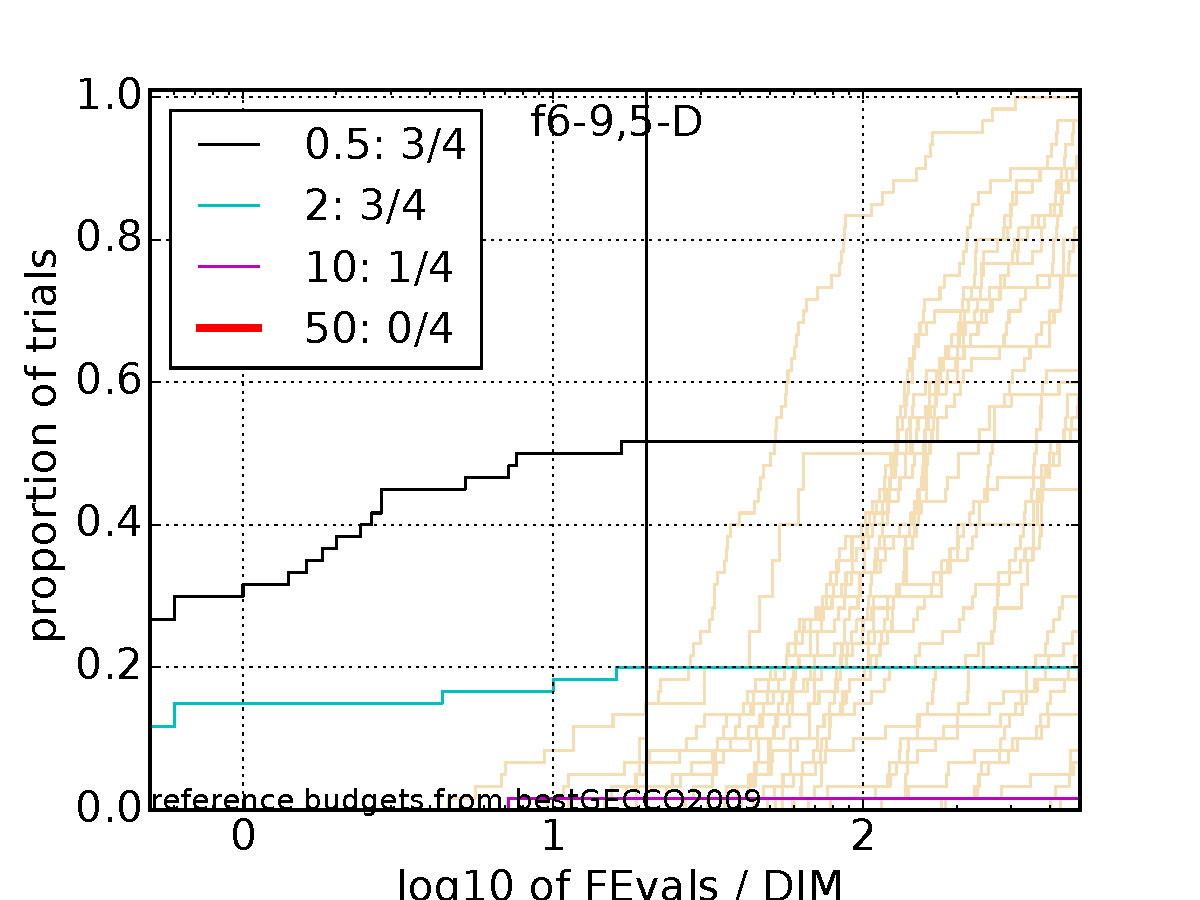
\includegraphics[width=0.268\textwidth,trim=0 0 0 13mm, clip]{pprldistr_05D_lcond} &
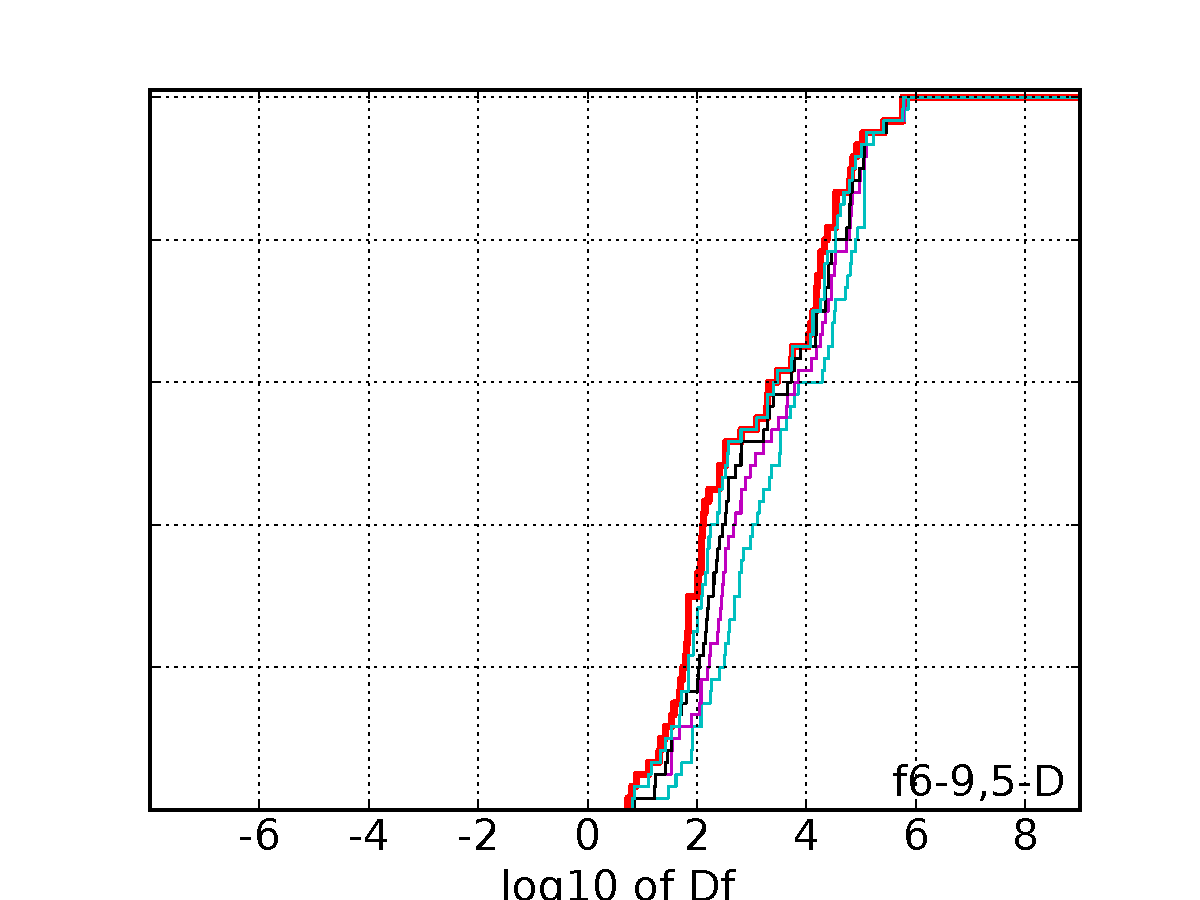
\includegraphics[width=0.2362\textwidth,trim=2.40cm 0 0 13mm, clip]{ppfvdistr_05D_lcond} &
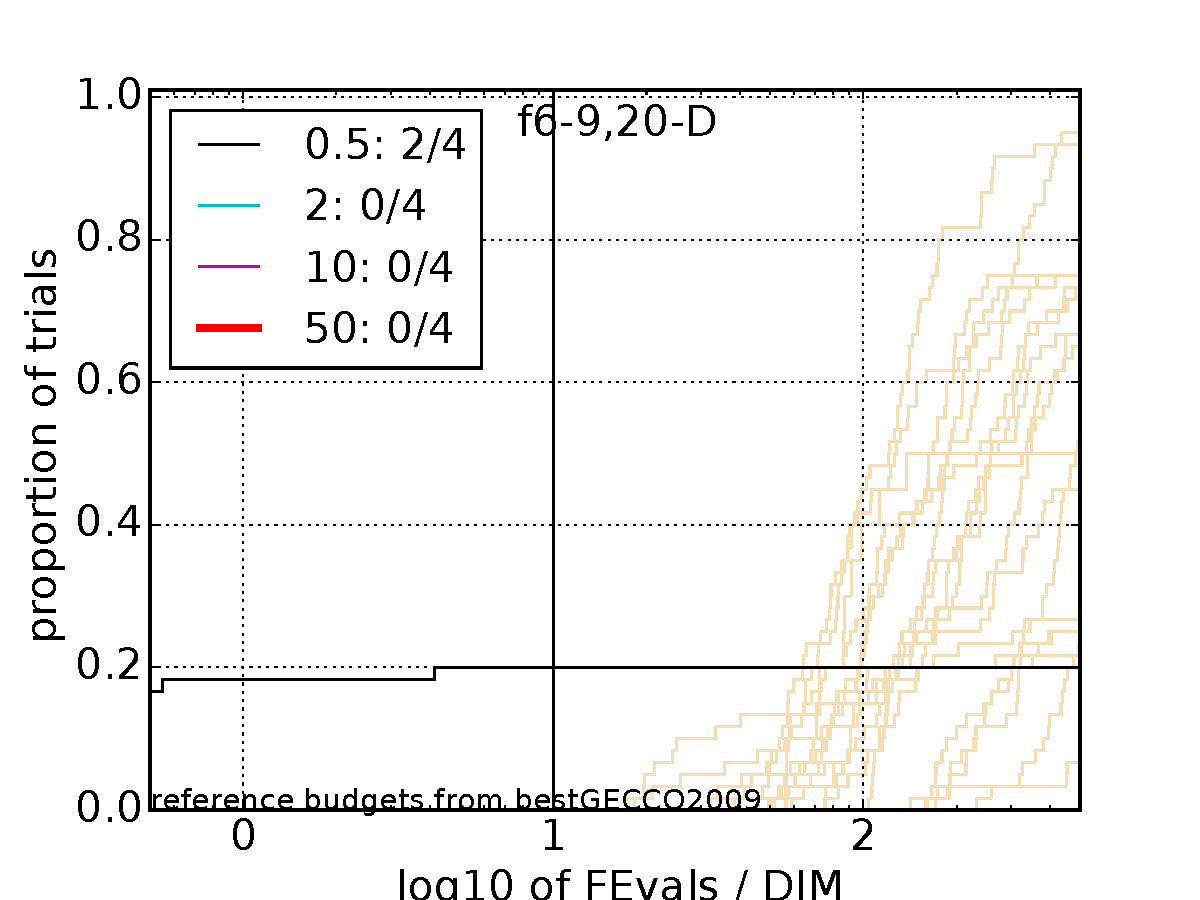
\includegraphics[width=0.268\textwidth,trim=0 0 0 13mm, clip]{pprldistr_20D_lcond} &
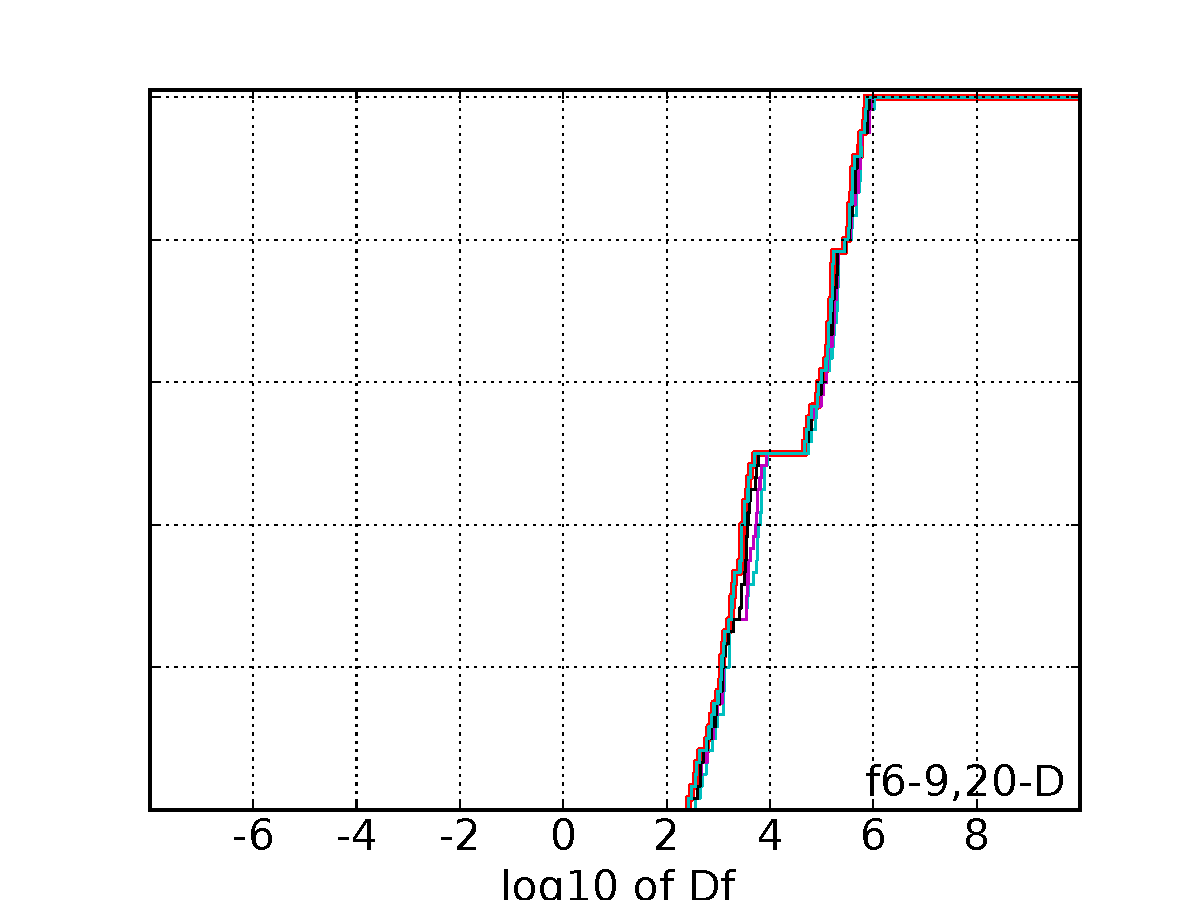
\includegraphics[width=0.2362\textwidth,trim=2.40cm 0 0 13mm, clip]{ppfvdistr_20D_lcond} \\[-2ex]
\rot[1.3]{ill-conditioned fcts}
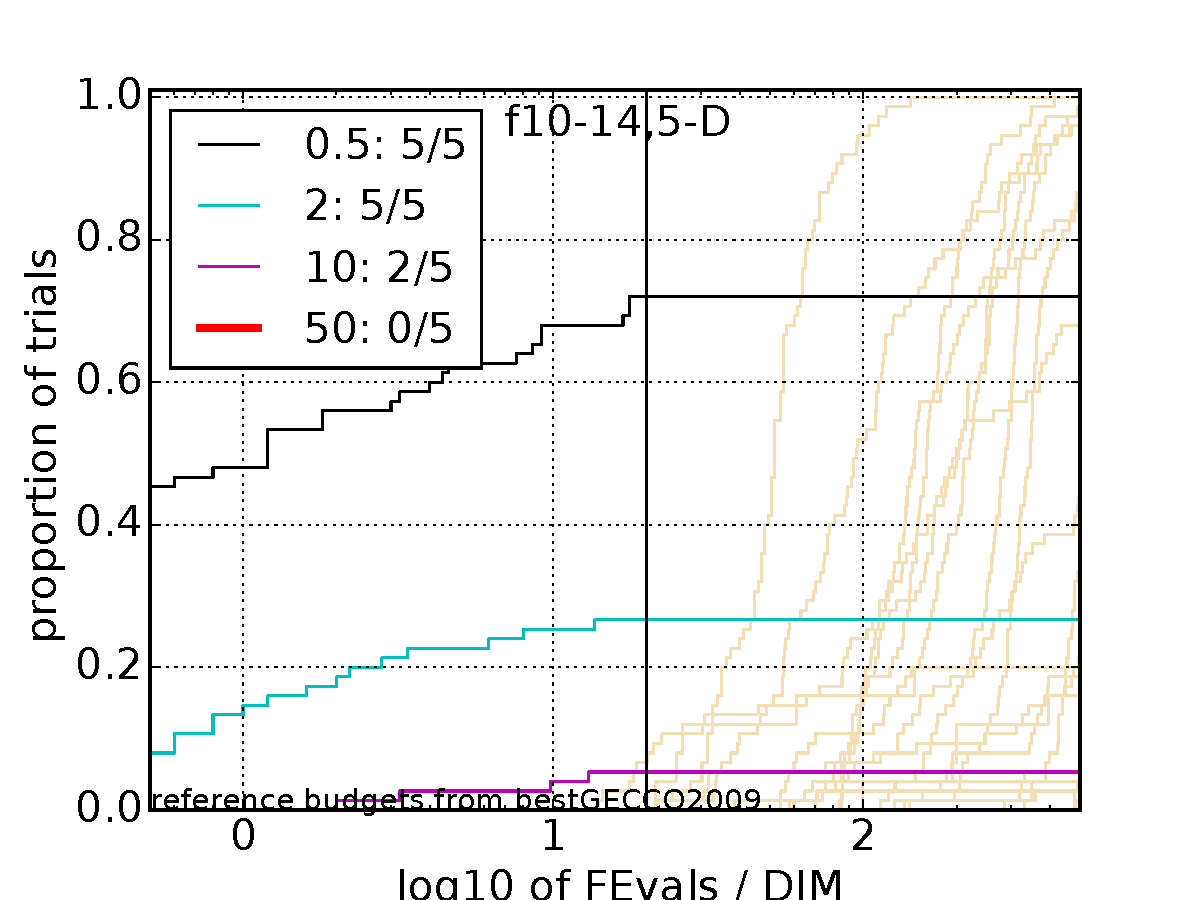
\includegraphics[width=0.268\textwidth,trim=0 0 0 13mm, clip]{pprldistr_05D_hcond} &
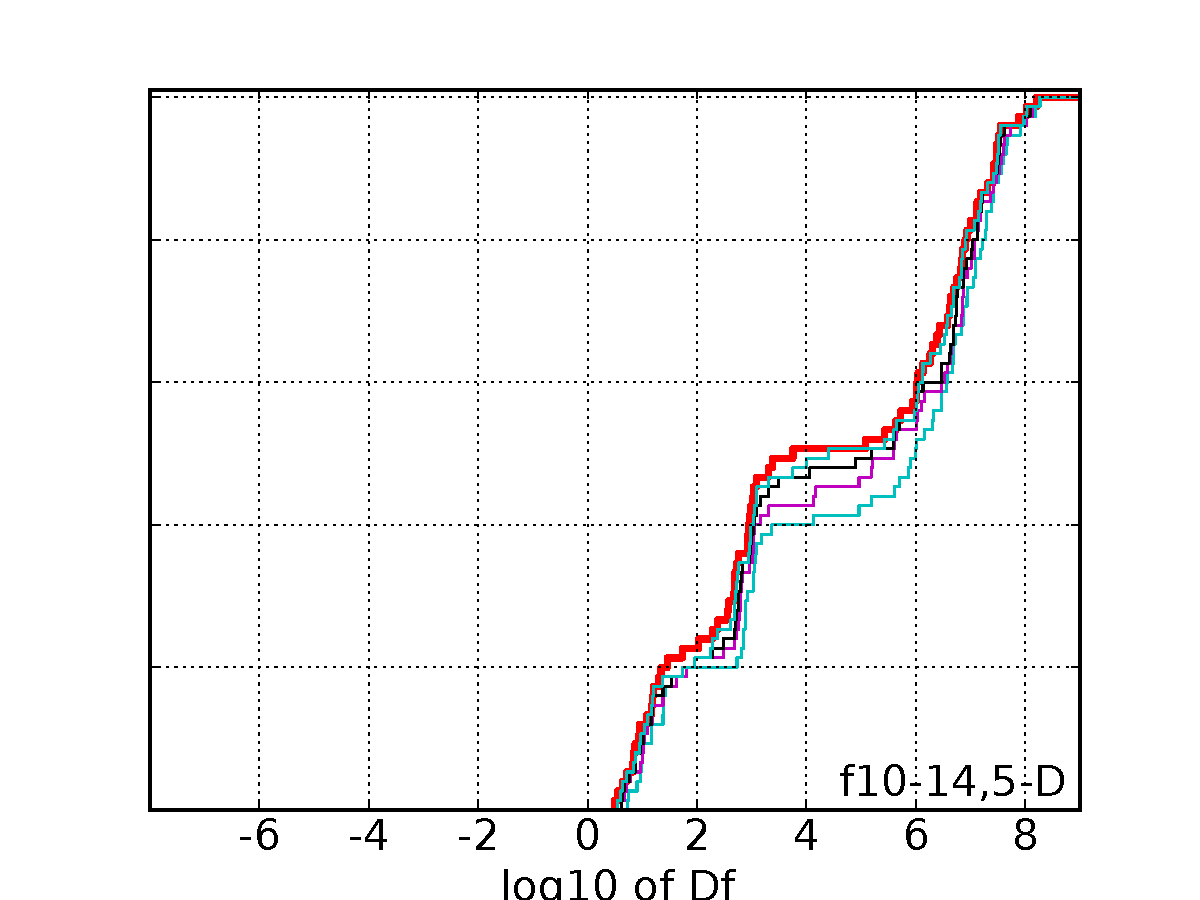
\includegraphics[width=0.2362\textwidth,trim=2.40cm 0 0 13mm, clip]{ppfvdistr_05D_hcond} &
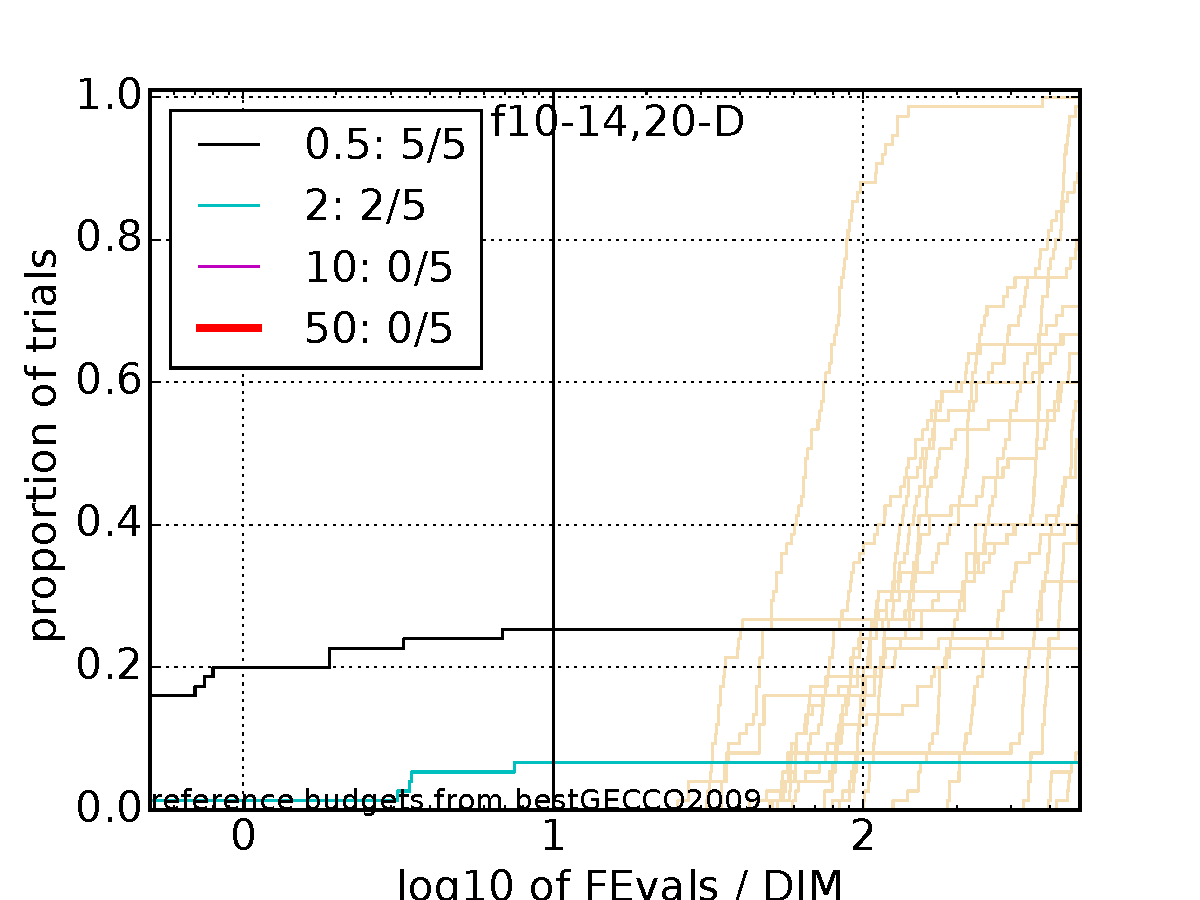
\includegraphics[width=0.268\textwidth,trim=0 0 0 13mm, clip]{pprldistr_20D_hcond} &
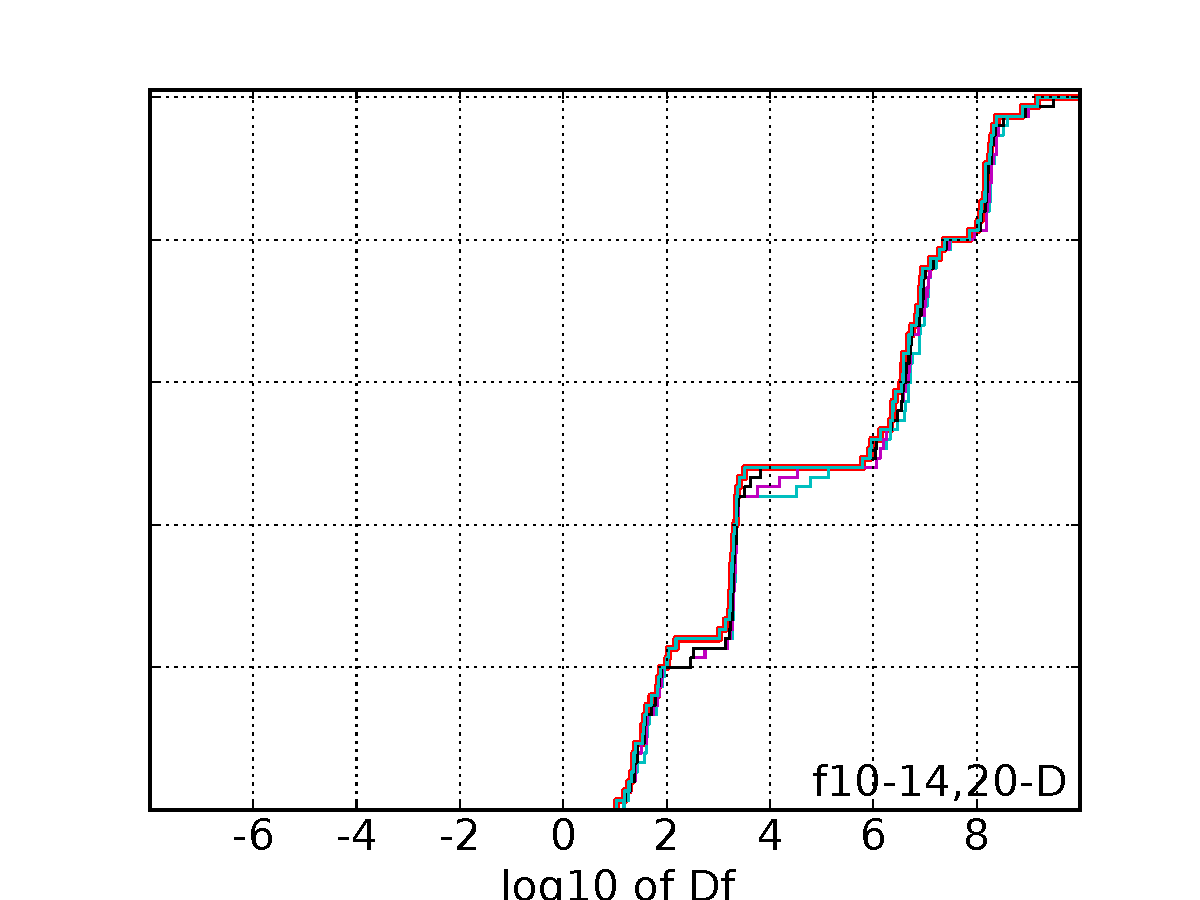
\includegraphics[width=0.2362\textwidth,trim=2.40cm 0 0 13mm, clip]{ppfvdistr_20D_hcond} \\[-2ex]
\rot[1.6]{multi-modal fcts}
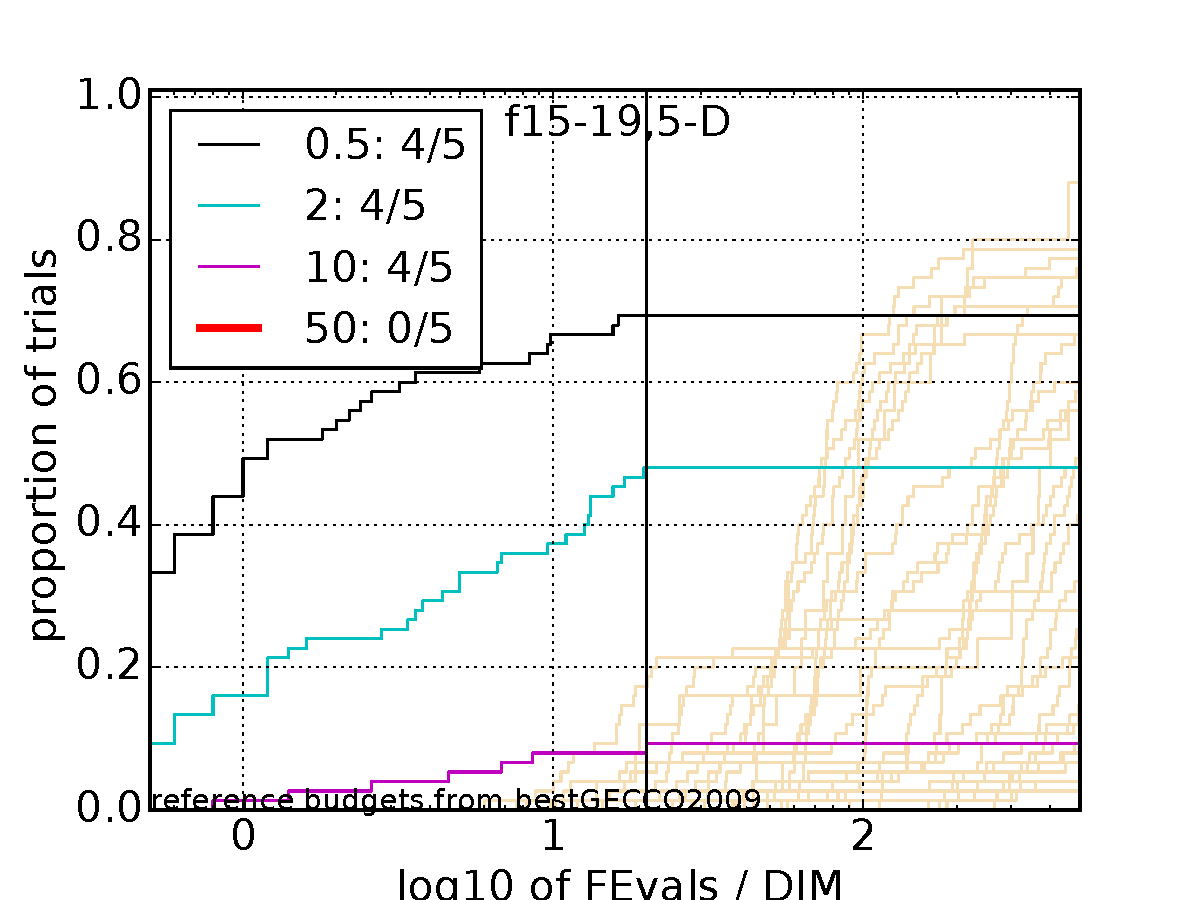
\includegraphics[width=0.268\textwidth,trim=0 0 0 13mm, clip]{pprldistr_05D_multi} &
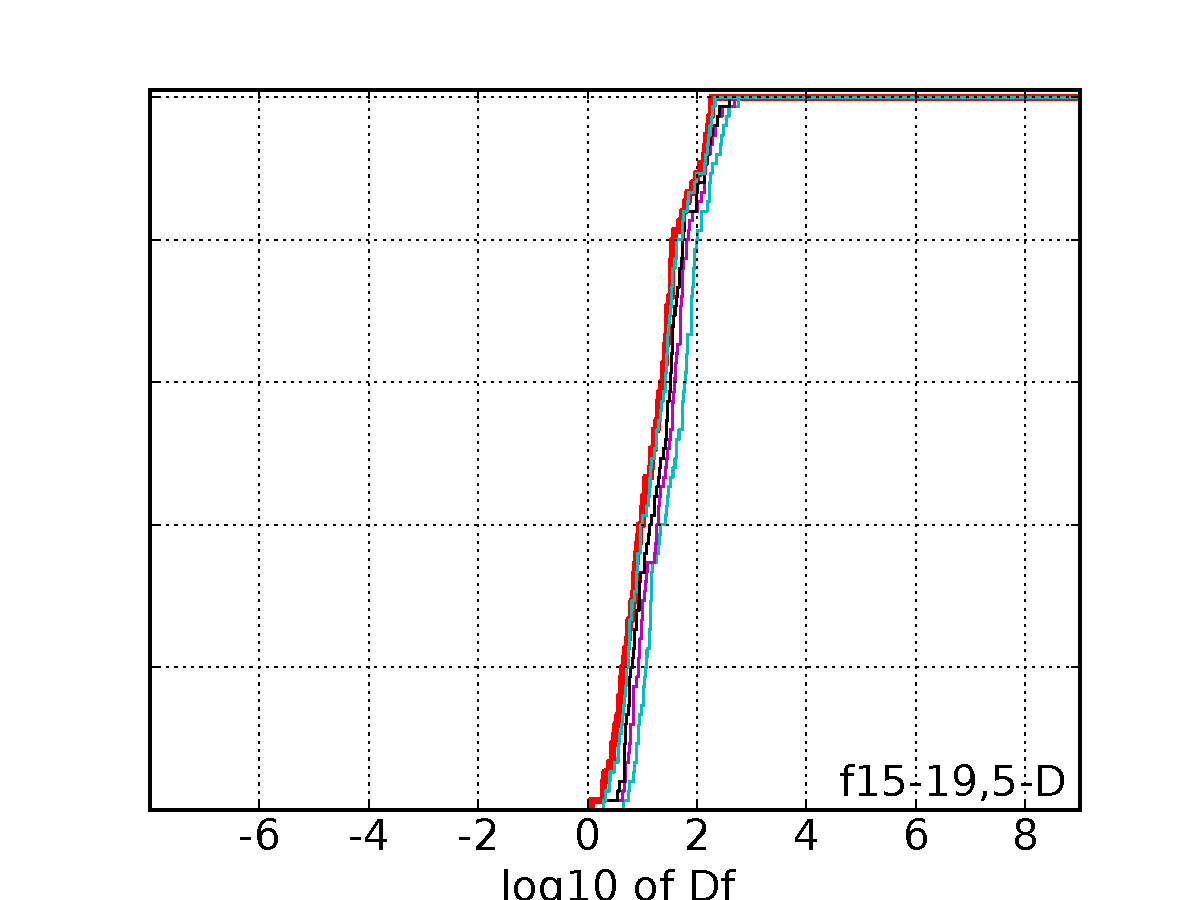
\includegraphics[width=0.2362\textwidth,trim=2.40cm 0 0 13mm, clip]{ppfvdistr_05D_multi} &
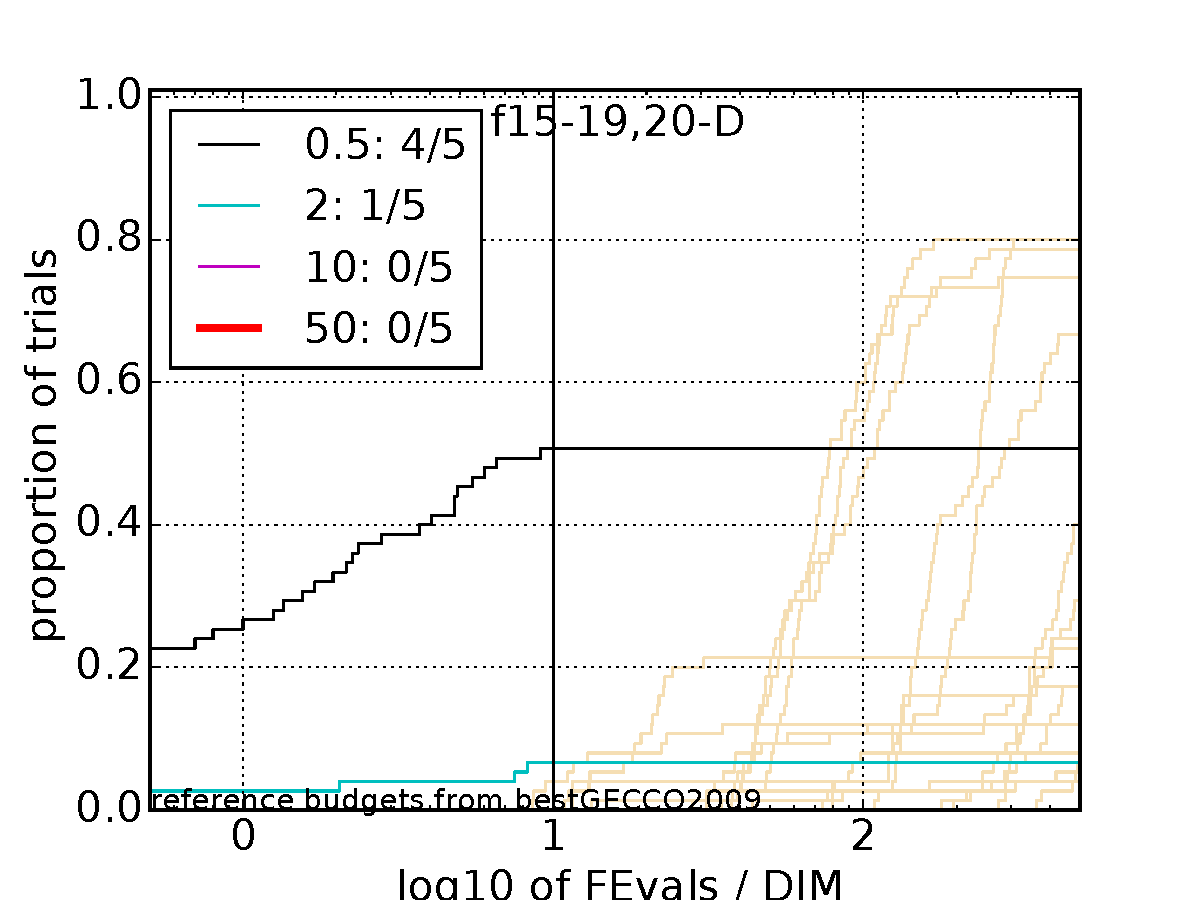
\includegraphics[width=0.268\textwidth,trim=0 0 0 13mm, clip]{pprldistr_20D_multi} &
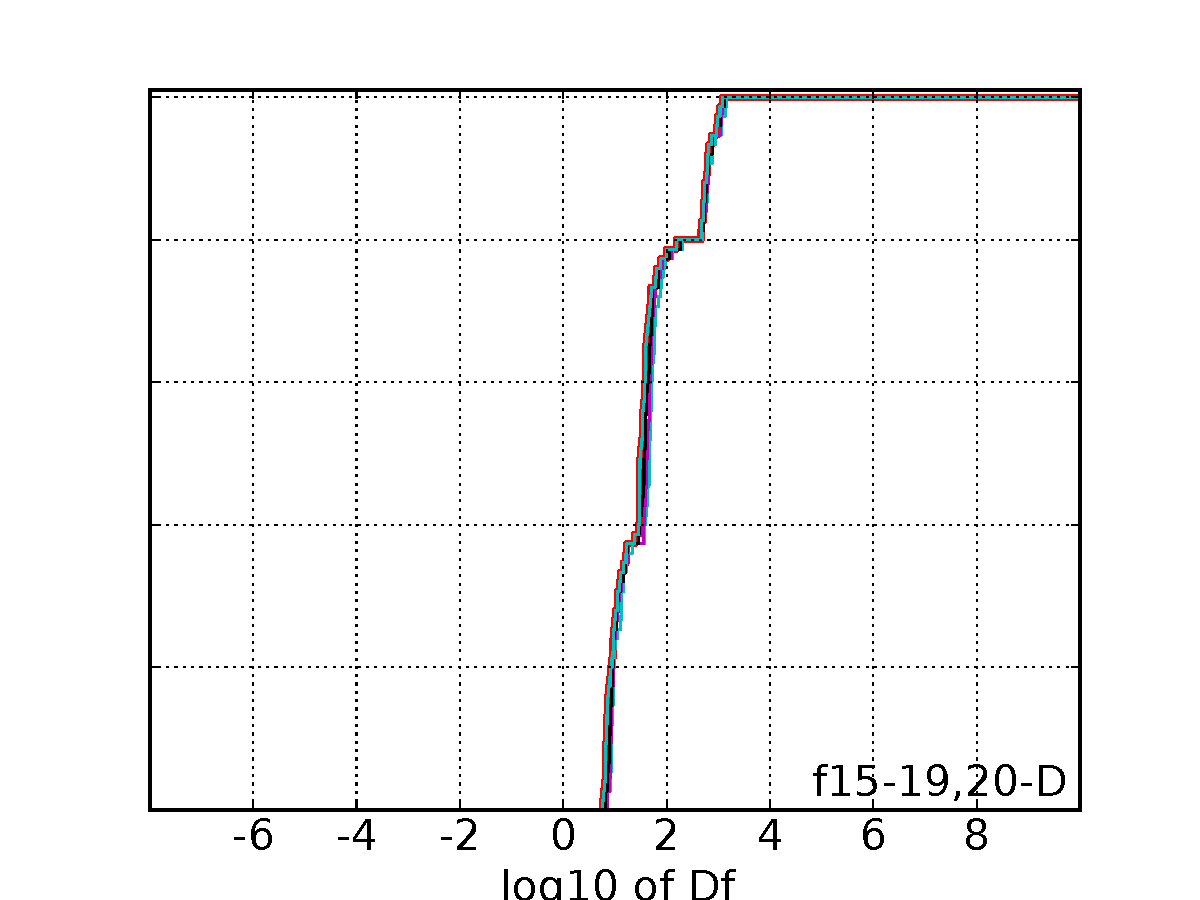
\includegraphics[width=0.2362\textwidth,trim=2.40cm 0 0 13mm, clip]{ppfvdistr_20D_multi} \\[-2ex]
\rot[1.0]{weak structure fcts}
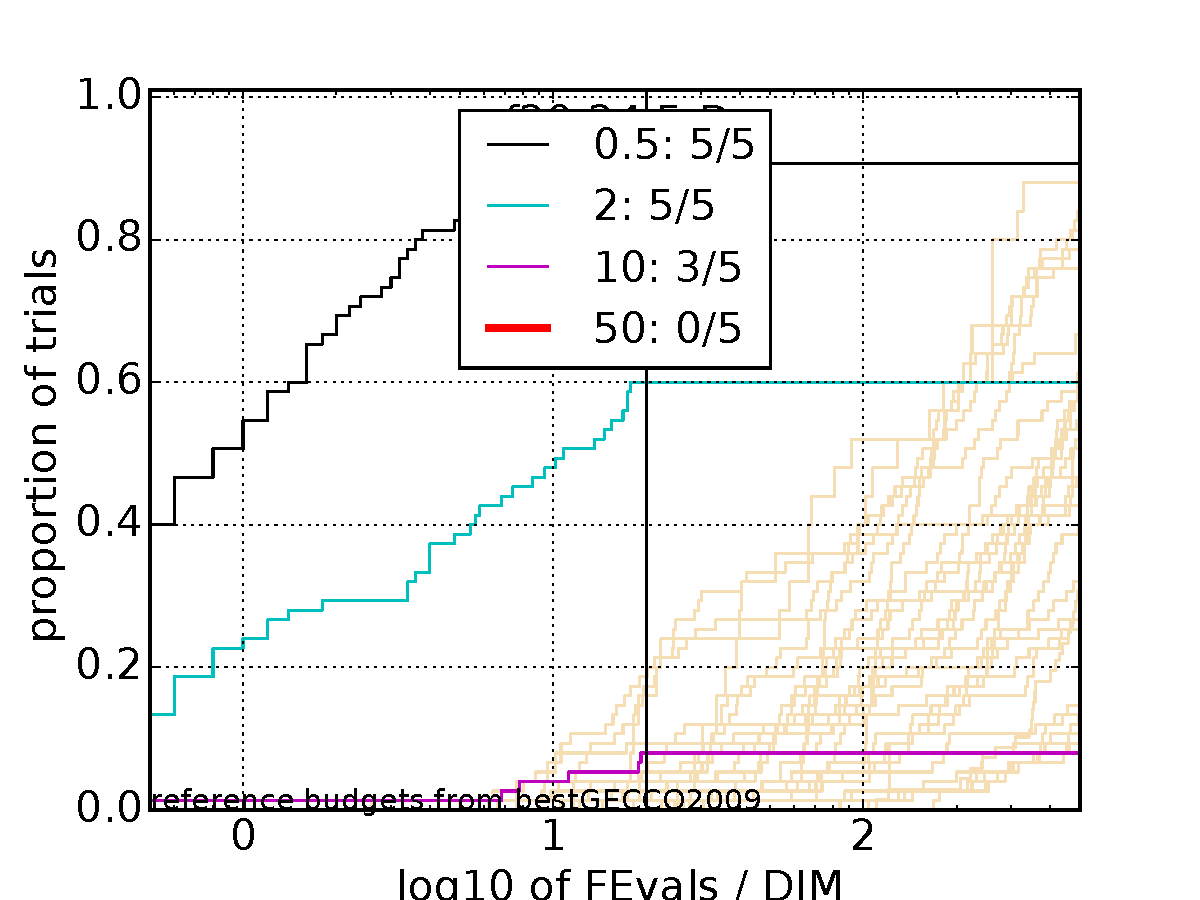
\includegraphics[width=0.268\textwidth,trim=0 0 0 13mm, clip]{pprldistr_05D_mult2} &
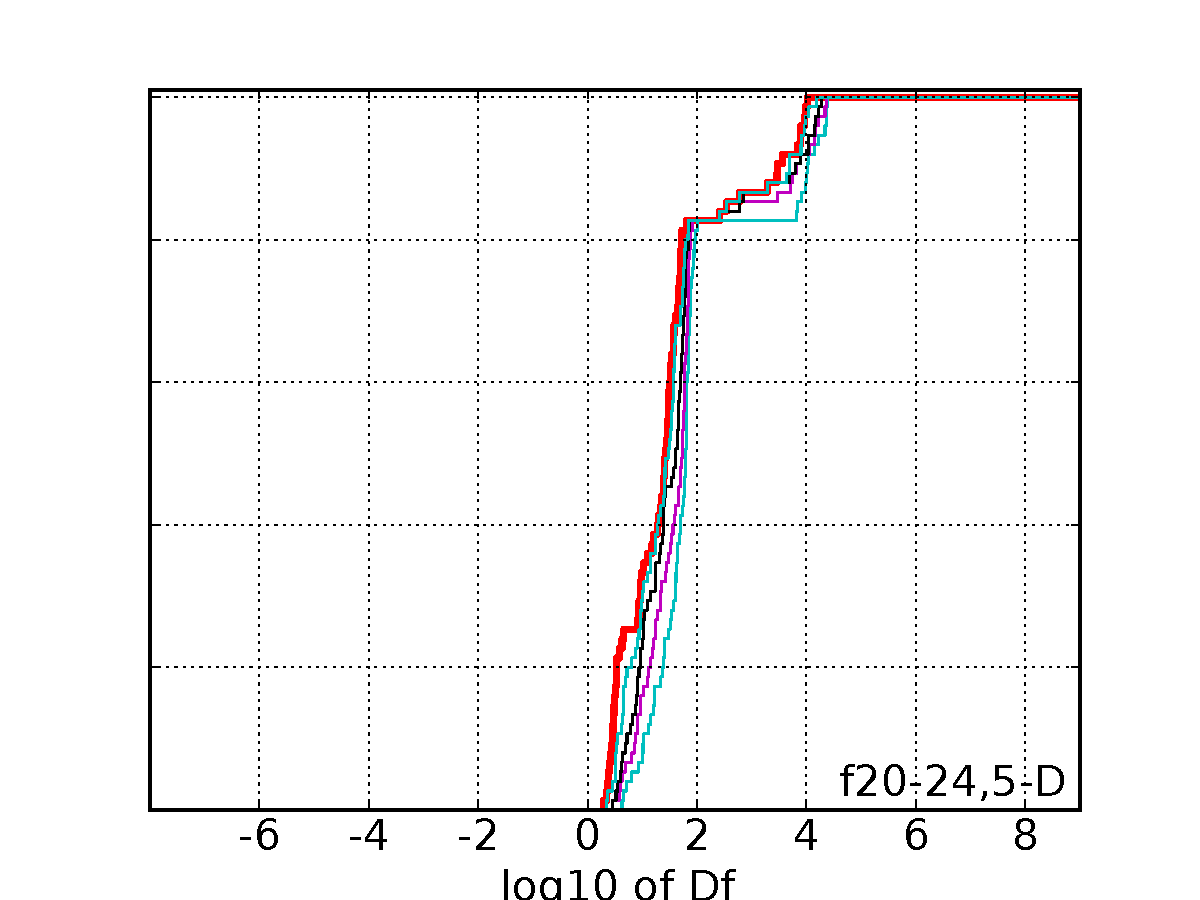
\includegraphics[width=0.2362\textwidth,trim=2.40cm 0 0 13mm, clip]{ppfvdistr_05D_mult2} &
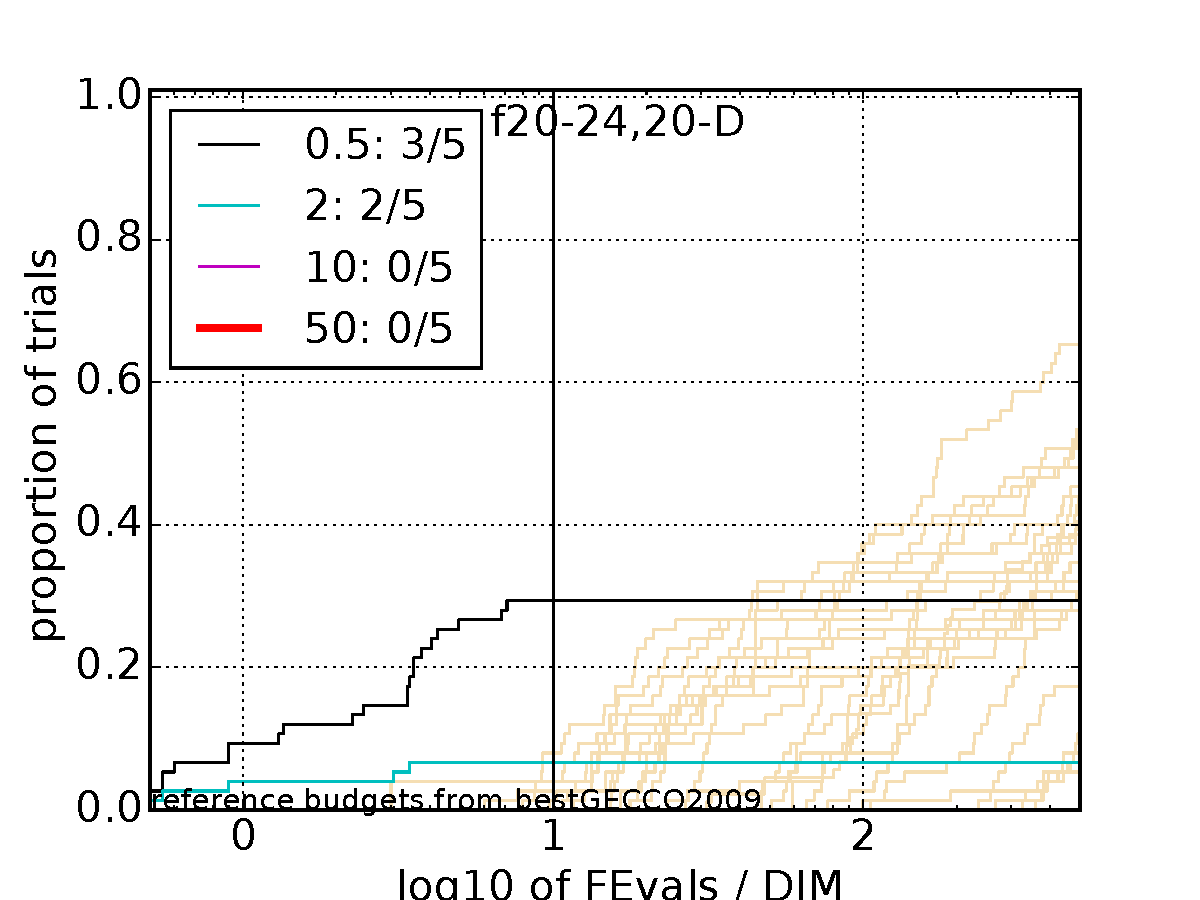
\includegraphics[width=0.268\textwidth,trim=0 0 0 13mm, clip]{pprldistr_20D_mult2} &
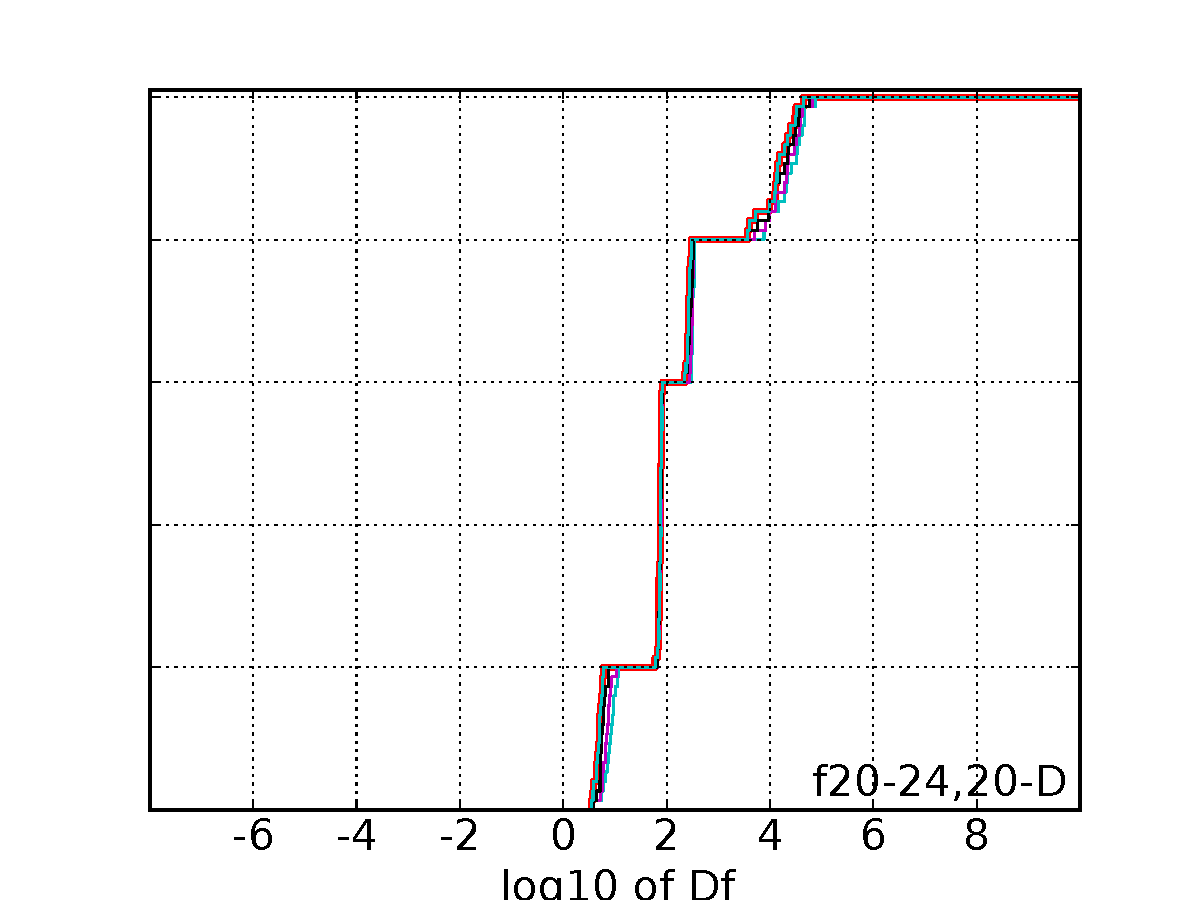
\includegraphics[width=0.2362\textwidth,trim=2.40cm 0 0 13mm, clip]{ppfvdistr_20D_mult2}\\[-2ex]
\rot{all functions}
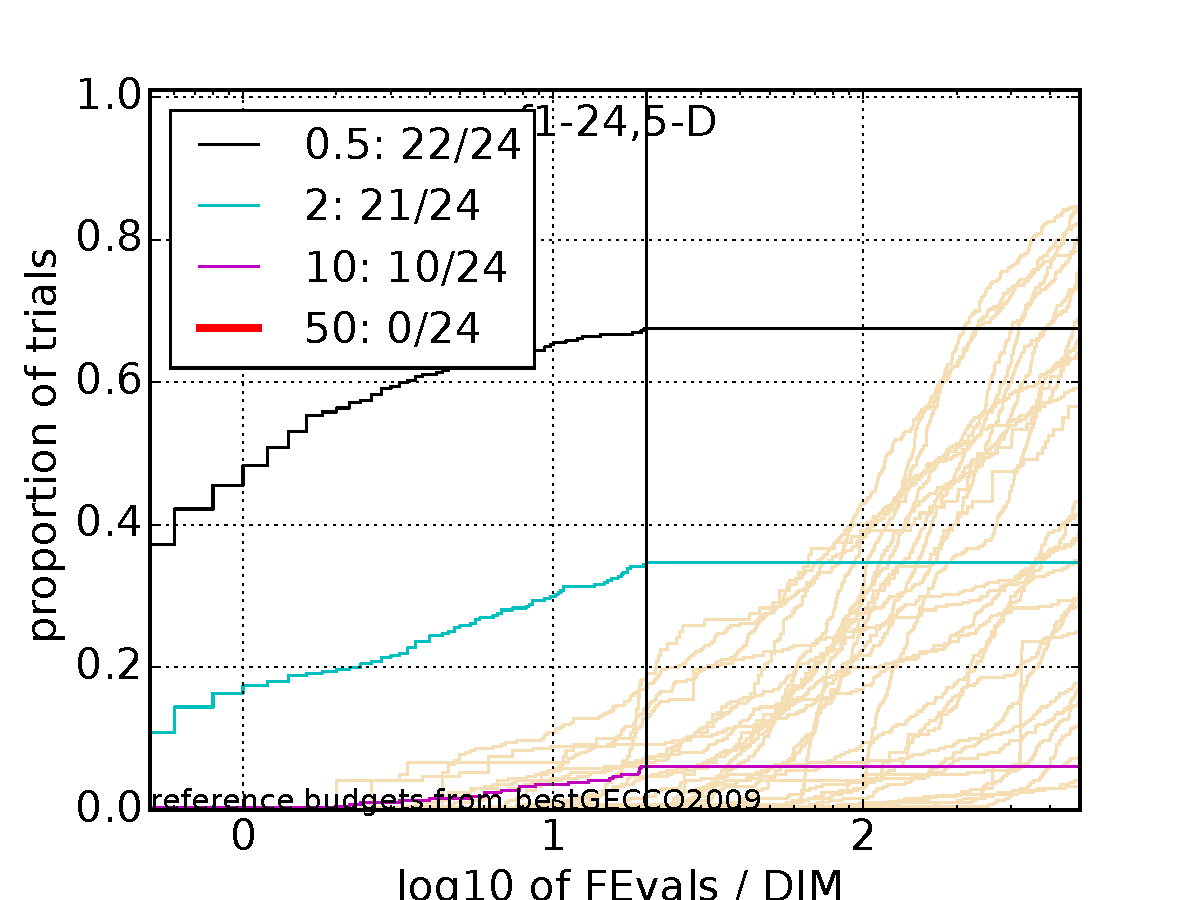
\includegraphics[width=0.268\textwidth,trim=0 0 0 13mm, clip]{pprldistr_05D_noiselessall} &
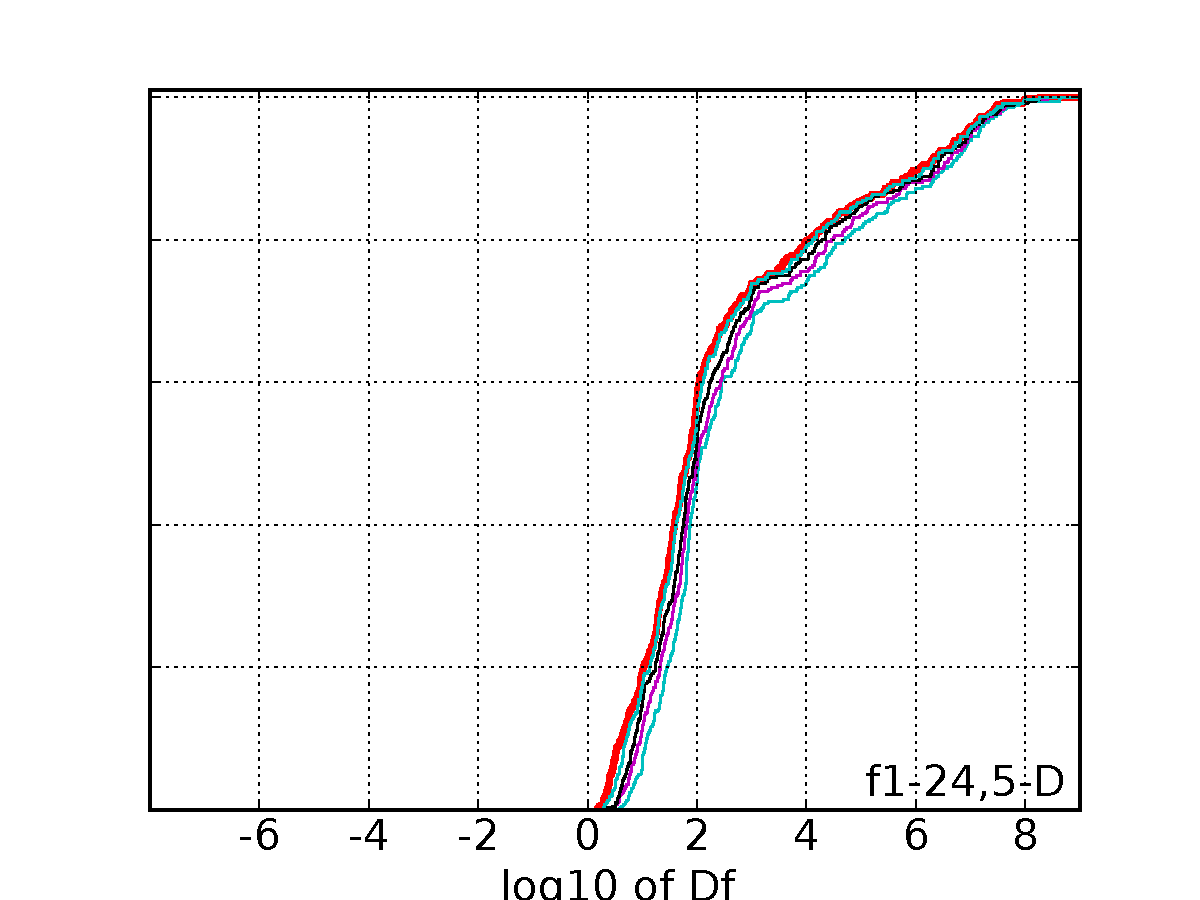
\includegraphics[width=0.2362\textwidth,trim=2.40cm 0 0 13mm, clip]{ppfvdistr_05D_noiselessall} &
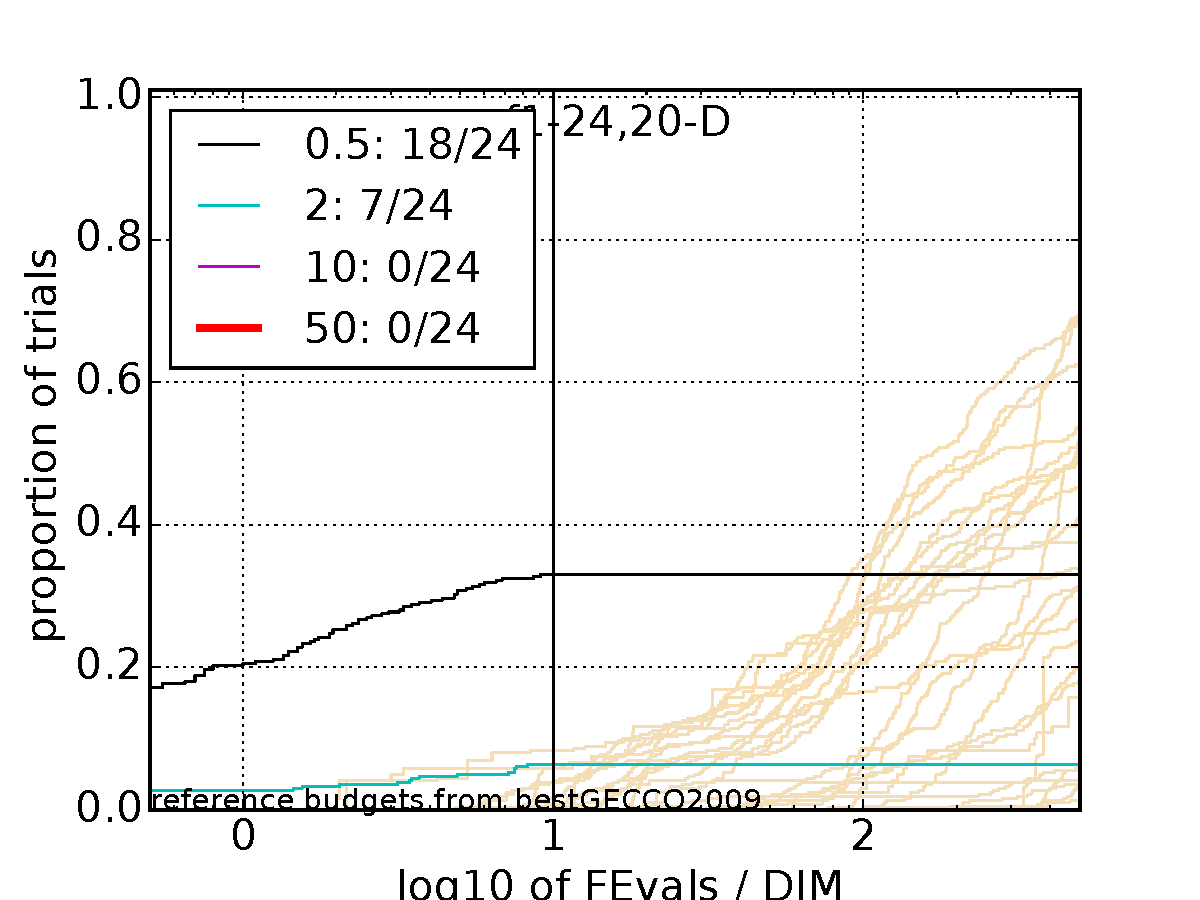
\includegraphics[width=0.268\textwidth,trim=0 0 0 13mm, clip]{pprldistr_20D_noiselessall} &
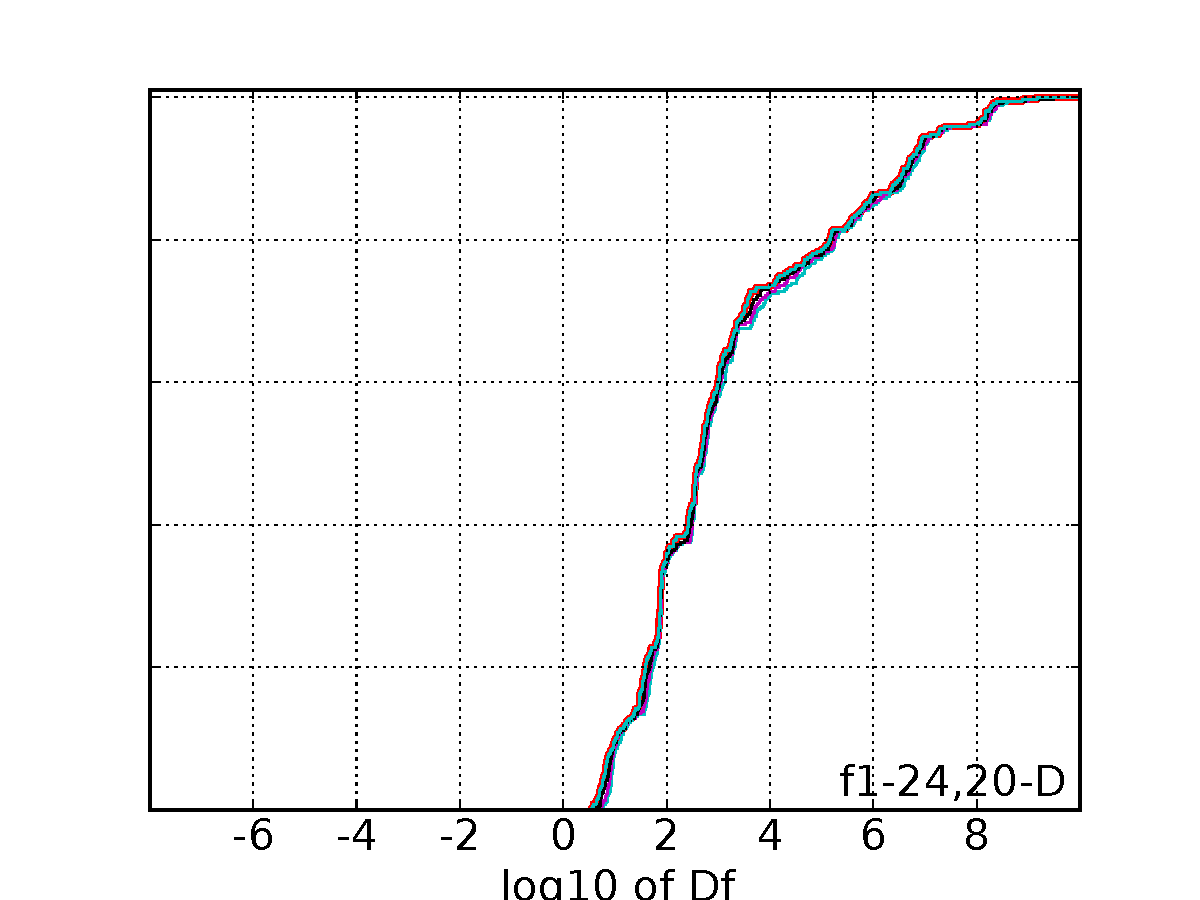
\includegraphics[width=0.2362\textwidth,trim=2.40cm 0 0 13mm, clip]{ppfvdistr_20D_noiselessall}
\vspace*{-0.5ex}
\end{tabular}
 \caption{\label{fig:RLDs}
 \bbobpprldistrlegend{}
 }
\end{figure*}
%%%%%%%%%%%%%%%%%%%%%%%%%%%%%%%%%%%%%%%%%%%%%%%%%%%%%%%%%%%%%%%%%%%%%%%%%%%%%%%


%%%%%%%%%%%%%%%%%%%%%%%%%%%%%%%%%%%%%%%%%%%%%%%%%%%%%%%%%%%%%%%%%%%%%%%%%%%%%%%
%%%%%%%%%%%%%%%%%%%%%%%%%%%%%%%%%%%%%%%%%%%%%%%%%%%%%%%%%%%%%%%%%%%%%%%%%%%%%%%

% ERT loss ratios (figure and table)

%%%%%%%%%%%%%%%%%%%%%%%%%%%%%%%%%%%%%%%%%%%%%%%%%%%%%%%%%%%%%%%%%%%%%%%%%%%%%%%
\begin{figure}
\centering
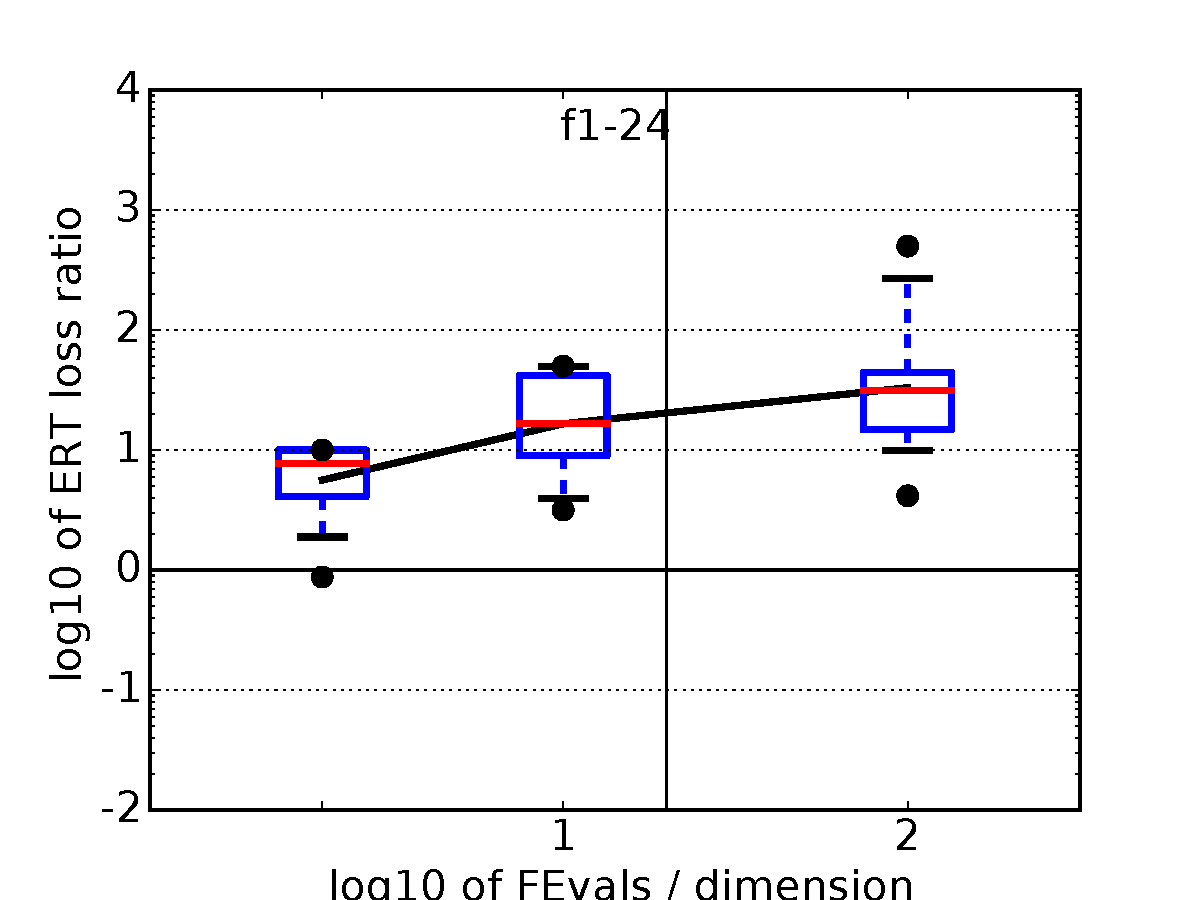
\includegraphics[width=0.24\textwidth,trim=0 0 16mm 12mm, clip]{pplogloss_05D_noiselessall}% 
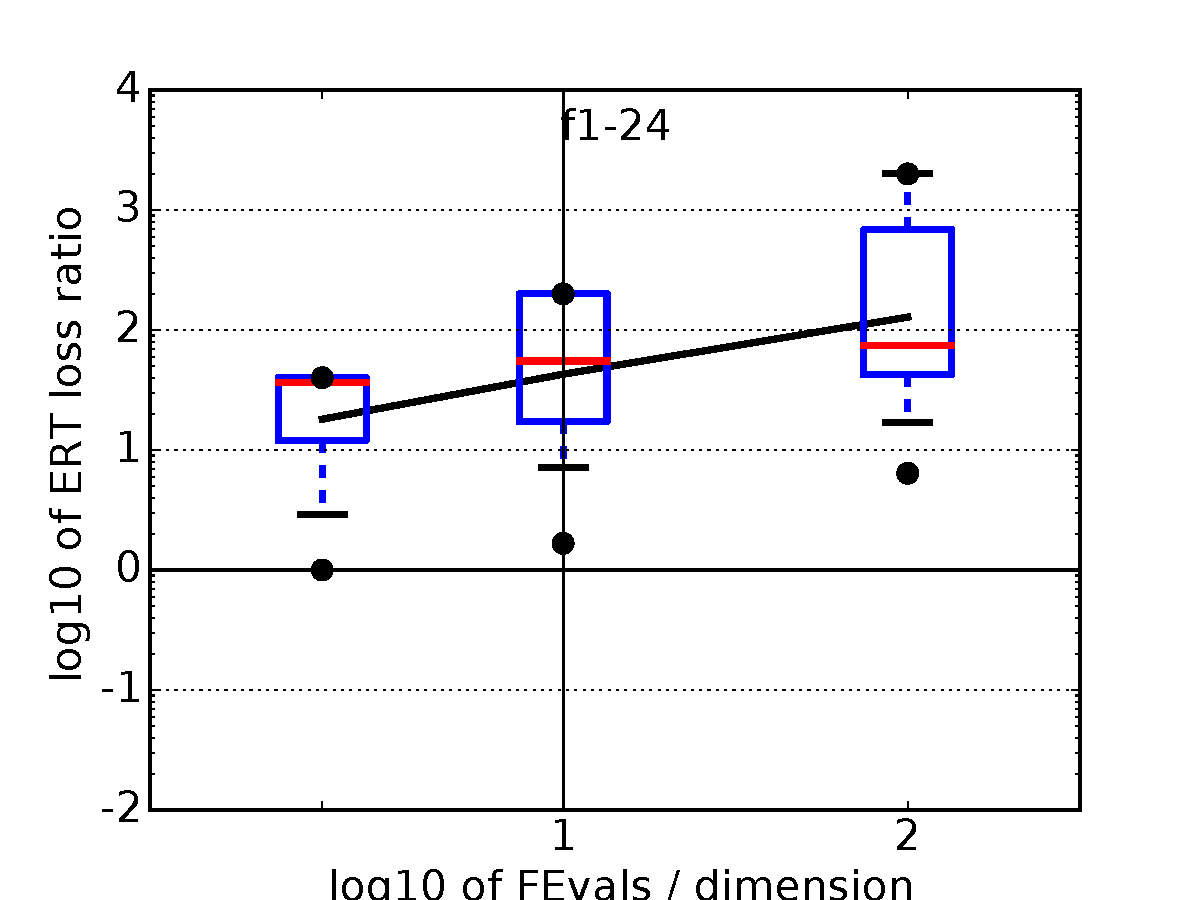
\includegraphics[width=0.24\textwidth,trim=7mm 0 9mm 12mm, clip]{pplogloss_20D_noiselessall}%
\\[-6.2ex]
\parbox{0.49\columnwidth}{\centering 5-D}%
\parbox{0.49\columnwidth}{\centering 20-D}\\[5ex]
%
\input{\bbobdatapath\algfolder pploglosstable_05D_noiselessall}\\
\input{\bbobdatapath\algfolder pploglosstable_20D_noiselessall}
\caption{\label{tab:ERTloss}%
\bbobloglosstablecaption{}
}
\end{figure}


%%%%%%%%%%%%%%%%%%%%%%%%%%%%%%%%%%%%%%%%%%%%%%%%%%%%%%%%%%%%%%%%%%%%%%%%%%%%%%%
%%%%%%%%%%%%%%%%%%%%%%%%%%%%%%%%%%%%%%%%%%%%%%%%%%%%%%%%%%%%%%%%%%%%%%%%%%%%%%%

% ERT loss ratios per function group

%%%%%%%%%%%%%%%%%%%%%%%%%%%%%%%%%%%%%%%%%%%%%%%%%%%%%%%%%%%%%%%%%%%%%%%%%%%%%%%
\begin{figure}
\begin{tabular}{@{}l@{}@{}l@{}}
\multicolumn{1}{c}{5-D} & \multicolumn{1}{c}{20-D}\\
\rot{separable fcts}
\hspace*{-2mm}
\includegraphics[width=0.24\textwidth,trim=0 0 16mm 12mm, clip]{pplogloss_05D_separ} &
\includegraphics[width=0.24\textwidth,trim=7mm 0 9mm 12mm, clip]{pplogloss_20D_separ}\\[-2ex]
\rot[2]{moderate fcts}
\hspace*{-2mm}
\includegraphics[width=0.24\textwidth,trim=0 0 16mm 12mm, clip]{pplogloss_05D_lcond} &
\includegraphics[width=0.24\textwidth,trim=7mm 0 9mm 12mm, clip]{pplogloss_20D_lcond}\\[-2ex]
\rot[1.3]{ill-conditioned fcts}
\hspace*{-2mm}
\includegraphics[width=0.24\textwidth,trim=0 0 16mm 12mm, clip]{pplogloss_05D_hcond} &
\includegraphics[width=0.24\textwidth,trim=7mm 0 9mm 12mm, clip]{pplogloss_20D_hcond}\\[-2ex]
\rot[1.6]{multi-modal fcts}
\hspace*{-2mm}
\includegraphics[width=0.24\textwidth,trim=0 0 16mm 12mm, clip]{pplogloss_05D_multi} &
\includegraphics[width=0.24\textwidth,trim=7mm 0 9mm 12mm, clip]{pplogloss_20D_multi}\\[-2ex]
\rot[1.0]{weak structure fcts}
\hspace*{-2mm}
\includegraphics[width=0.24\textwidth,trim=0 0 16mm 12mm, clip]{pplogloss_05D_mult2} &
\includegraphics[width=0.24\textwidth,trim=7mm 0 9mm 12mm, clip]{pplogloss_20D_mult2}
\vspace*{-0.5ex}
\end{tabular}
 \caption{\label{fig:ERTlogloss}%
\bbobloglossfigurecaption{}
}
\end{figure}
\clearpage

%%%%%%%%%%%%%%%%%%%%%%%%%%%%%%%%%%%%%%%%%%%%%%%%%%%%%%%%%%%%%%%%%%%%%%%%%%%%%%%
%%%%%%%%%%%%%%%%%%%%%%%%%%%%%%%%%%%%%%%%%%%%%%%%%%%%%%%%%%%%%%%%%%%%%%%%%%%%%%%


% use section* for acknowledgement
\section*{Acknowledgment}
The authors would like to thank...



%%%%%%%%%%%%%%%%%%%%%%%%%%%%%%%%%%%%%%%%%%%%%%%%%%%%%%%%%%%%%%%%%%%%%%%%%%%%%%%
%%%%%%%%%%%%%%%%%%%%%%%%%%%%%%%%%%%%%%%%%%%%%%%%%%%%%%%%%%%%%%%%%%%%%%%%%%%%%%%

% trigger a \newpage just before the given reference
% number - used to balance the columns on the last page
% adjust value as needed - may need to be readjusted if
% the document is modified later
%\IEEEtriggeratref{8}
% The "triggered" command can be changed if desired:
%\IEEEtriggercmd{\enlargethispage{-5in}}

% references section

% can use a bibliography generated by BibTeX as a .bbl file
% BibTeX documentation can be easily obtained at:
% http://www.ctan.org/tex-archive/biblio/bibtex/contrib/doc/
% The IEEEtran BibTeX style support page is at:
% http://www.michaelshell.org/tex/ieeetran/bibtex/
\bibliographystyle{IEEEtran}
% argument is your BibTeX string definitions and bibliography database(s)
\bibliography{bbob}  % bbob.bib is the name of the Bibliography in this case
%
% <OR> manually copy in the resultant .bbl file
% set second argument of \begin to the number of references
% (used to reserve space for the reference number labels box)
%\begin{thebibliography}{1}
%
%\bibitem{IEEEhowto:kopka}
%H.~Kopka and P.~W. Daly, \emph{A Guide to \LaTeX}, 3rd~ed.\hskip 1em plus
%  0.5em minus 0.4em\relax Harlow, England: Addison-Wesley, 1999.
%
%\end{thebibliography}


% that's all folks
\end{document}


